\documentclass[twoside]{book}

% Packages required by doxygen
\usepackage{fixltx2e}
\usepackage{calc}
\usepackage{doxygen}
\usepackage[export]{adjustbox} % also loads graphicx
\usepackage{graphicx}
\usepackage[utf8]{inputenc}
\usepackage{makeidx}
\usepackage{multicol}
\usepackage{multirow}
\PassOptionsToPackage{warn}{textcomp}
\usepackage{textcomp}
\usepackage[nointegrals]{wasysym}
\usepackage[table]{xcolor}

% Font selection
\usepackage[T1]{fontenc}
\usepackage[scaled=.90]{helvet}
\usepackage{courier}
\usepackage{amssymb}
\usepackage{sectsty}
\renewcommand{\familydefault}{\sfdefault}
\allsectionsfont{%
  \fontseries{bc}\selectfont%
  \color{darkgray}%
}
\renewcommand{\DoxyLabelFont}{%
  \fontseries{bc}\selectfont%
  \color{darkgray}%
}
\newcommand{\+}{\discretionary{\mbox{\scriptsize$\hookleftarrow$}}{}{}}

% Page & text layout
\usepackage{geometry}
\geometry{%
  a4paper,%
  top=2.5cm,%
  bottom=2.5cm,%
  left=2.5cm,%
  right=2.5cm%
}
\tolerance=750
\hfuzz=15pt
\hbadness=750
\setlength{\emergencystretch}{15pt}
\setlength{\parindent}{0cm}
\setlength{\parskip}{3ex plus 2ex minus 2ex}
\makeatletter
\renewcommand{\paragraph}{%
  \@startsection{paragraph}{4}{0ex}{-1.0ex}{1.0ex}{%
    \normalfont\normalsize\bfseries\SS@parafont%
  }%
}
\renewcommand{\subparagraph}{%
  \@startsection{subparagraph}{5}{0ex}{-1.0ex}{1.0ex}{%
    \normalfont\normalsize\bfseries\SS@subparafont%
  }%
}
\makeatother

% Headers & footers
\usepackage{fancyhdr}
\pagestyle{fancyplain}
\fancyhead[LE]{\fancyplain{}{\bfseries\thepage}}
\fancyhead[CE]{\fancyplain{}{}}
\fancyhead[RE]{\fancyplain{}{\bfseries\leftmark}}
\fancyhead[LO]{\fancyplain{}{\bfseries\rightmark}}
\fancyhead[CO]{\fancyplain{}{}}
\fancyhead[RO]{\fancyplain{}{\bfseries\thepage}}
\fancyfoot[LE]{\fancyplain{}{}}
\fancyfoot[CE]{\fancyplain{}{}}
\fancyfoot[RE]{\fancyplain{}{\bfseries\scriptsize Generated by Doxygen }}
\fancyfoot[LO]{\fancyplain{}{\bfseries\scriptsize Generated by Doxygen }}
\fancyfoot[CO]{\fancyplain{}{}}
\fancyfoot[RO]{\fancyplain{}{}}
\renewcommand{\footrulewidth}{0.4pt}
\renewcommand{\chaptermark}[1]{%
  \markboth{#1}{}%
}
\renewcommand{\sectionmark}[1]{%
  \markright{\thesection\ #1}%
}

% Indices & bibliography
\usepackage{natbib}
\usepackage[titles]{tocloft}
\setcounter{tocdepth}{3}
\setcounter{secnumdepth}{5}
\makeindex

% Hyperlinks (required, but should be loaded last)
\usepackage{ifpdf}
\ifpdf
  \usepackage[pdftex,pagebackref=true]{hyperref}
\else
  \usepackage[ps2pdf,pagebackref=true]{hyperref}
\fi
\hypersetup{%
  colorlinks=true,%
  linkcolor=blue,%
  citecolor=blue,%
  unicode%
}

% Custom commands
\newcommand{\clearemptydoublepage}{%
  \newpage{\pagestyle{empty}\cleardoublepage}%
}

\usepackage{caption}
\captionsetup{labelsep=space,justification=centering,font={bf},singlelinecheck=off,skip=4pt,position=top}

%===== C O N T E N T S =====

\begin{document}

% Titlepage & ToC
\hypersetup{pageanchor=false,
             bookmarksnumbered=true,
             pdfencoding=unicode
            }
\pagenumbering{alph}
\begin{titlepage}
\vspace*{7cm}
\begin{center}%
{\Large Easyuino \\[1ex]\large 1.\+1.\+0 }\\
\vspace*{1cm}
{\large Generated by Doxygen 1.8.13}\\
\end{center}
\end{titlepage}
\clearemptydoublepage
\pagenumbering{roman}
\tableofcontents
\clearemptydoublepage
\pagenumbering{arabic}
\hypersetup{pageanchor=true}

%--- Begin generated contents ---
\chapter{Hierarchical Index}
\section{Class Hierarchy}
This inheritance list is sorted roughly, but not completely, alphabetically\+:\begin{DoxyCompactList}
\item \contentsline{section}{Easyuino\+:\+:Device}{\pageref{class_easyuino_1_1_device}}{}
\begin{DoxyCompactList}
\item \contentsline{section}{Easyuino\+:\+:Distance\+Meter}{\pageref{class_easyuino_1_1_distance_meter}}{}
\begin{DoxyCompactList}
\item \contentsline{section}{Easyuino\+:\+:Distance\+Meter\+Non\+Block}{\pageref{class_easyuino_1_1_distance_meter_non_block}}{}
\begin{DoxyCompactList}
\item \contentsline{section}{Easyuino\+:\+:Distance\+Meter\+Accurate}{\pageref{class_easyuino_1_1_distance_meter_accurate}}{}
\end{DoxyCompactList}
\item \contentsline{section}{Easyuino\+:\+:Distance\+Meter\+Printable}{\pageref{class_easyuino_1_1_distance_meter_printable}}{}
\end{DoxyCompactList}
\item \contentsline{section}{Easyuino\+:\+:G\+S\+M\+Service}{\pageref{class_easyuino_1_1_g_s_m_service}}{}
\begin{DoxyCompactList}
\item \contentsline{section}{Easyuino\+:\+:G\+S\+M\+Service\+Secure}{\pageref{class_easyuino_1_1_g_s_m_service_secure}}{}
\end{DoxyCompactList}
\item \contentsline{section}{Easyuino\+:\+:Infra\+Red\+Receiver}{\pageref{class_easyuino_1_1_infra_red_receiver}}{}
\item \contentsline{section}{Easyuino\+:\+:Relay}{\pageref{class_easyuino_1_1_relay}}{}
\begin{DoxyCompactList}
\item \contentsline{section}{Easyuino\+:\+:Relay\+Named}{\pageref{class_easyuino_1_1_relay_named}}{}
\end{DoxyCompactList}
\item \contentsline{section}{Easyuino\+:\+:R\+G\+B\+Led}{\pageref{class_easyuino_1_1_r_g_b_led}}{}
\item \contentsline{section}{Easyuino\+:\+:Seven\+Segments}{\pageref{class_easyuino_1_1_seven_segments}}{}
\item \contentsline{section}{Easyuino\+:\+:Water\+Detector}{\pageref{class_easyuino_1_1_water_detector}}{}
\item \contentsline{section}{Easyuino\+:\+:Water\+Flow\+Sensor}{\pageref{class_easyuino_1_1_water_flow_sensor}}{}
\begin{DoxyCompactList}
\item \contentsline{section}{Easyuino\+:\+:Water\+Flow\+Meter}{\pageref{class_easyuino_1_1_water_flow_meter}}{}
\end{DoxyCompactList}
\end{DoxyCompactList}
\item \contentsline{section}{Easyuino\+:\+:Printable}{\pageref{class_easyuino_1_1_printable}}{}
\begin{DoxyCompactList}
\item \contentsline{section}{Easyuino\+:\+:Distance\+Meter\+Printable}{\pageref{class_easyuino_1_1_distance_meter_printable}}{}
\item \contentsline{section}{Easyuino\+:\+:Relay\+Named}{\pageref{class_easyuino_1_1_relay_named}}{}
\end{DoxyCompactList}
\item \contentsline{section}{Easyuino\+:\+:S\+MS}{\pageref{class_easyuino_1_1_s_m_s}}{}
\item \contentsline{section}{Easyuino\+:\+:Utilities}{\pageref{class_easyuino_1_1_utilities}}{}
\end{DoxyCompactList}

\chapter{Class Index}
\section{Class List}
Here are the classes, structs, unions and interfaces with brief descriptions\+:\begin{DoxyCompactList}
\item\contentsline{section}{\hyperlink{class_easyuino_1_1_device}{Easyuino\+::\+Device} }{\pageref{class_easyuino_1_1_device}}{}
\item\contentsline{section}{\hyperlink{class_easyuino_1_1_distance_meter}{Easyuino\+::\+Distance\+Meter} }{\pageref{class_easyuino_1_1_distance_meter}}{}
\item\contentsline{section}{\hyperlink{class_easyuino_1_1_distance_meter_accurate}{Easyuino\+::\+Distance\+Meter\+Accurate} }{\pageref{class_easyuino_1_1_distance_meter_accurate}}{}
\item\contentsline{section}{\hyperlink{class_distance_meter_accurate_test}{Distance\+Meter\+Accurate\+Test} }{\pageref{class_distance_meter_accurate_test}}{}
\item\contentsline{section}{\hyperlink{class_easyuino_1_1_distance_meter_non_block}{Easyuino\+::\+Distance\+Meter\+Non\+Block} }{\pageref{class_easyuino_1_1_distance_meter_non_block}}{}
\item\contentsline{section}{\hyperlink{class_distance_meter_non_block_test}{Distance\+Meter\+Non\+Block\+Test} }{\pageref{class_distance_meter_non_block_test}}{}
\item\contentsline{section}{\hyperlink{class_easyuino_1_1_distance_meter_printable}{Easyuino\+::\+Distance\+Meter\+Printable} }{\pageref{class_easyuino_1_1_distance_meter_printable}}{}
\item\contentsline{section}{\hyperlink{class_distance_meter_test}{Distance\+Meter\+Test} }{\pageref{class_distance_meter_test}}{}
\item\contentsline{section}{\hyperlink{class_easyuino_1_1_g_s_m_service}{Easyuino\+::\+G\+S\+M\+Service} }{\pageref{class_easyuino_1_1_g_s_m_service}}{}
\item\contentsline{section}{\hyperlink{class_easyuino_1_1_g_s_m_service_secure}{Easyuino\+::\+G\+S\+M\+Service\+Secure} }{\pageref{class_easyuino_1_1_g_s_m_service_secure}}{}
\item\contentsline{section}{\hyperlink{class_easyuino_1_1_infra_red_receiver}{Easyuino\+::\+Infra\+Red\+Receiver} }{\pageref{class_easyuino_1_1_infra_red_receiver}}{}
\item\contentsline{section}{\hyperlink{class_manual_test}{Manual\+Test} }{\pageref{class_manual_test}}{}
\item\contentsline{section}{\hyperlink{class_easyuino_1_1_printable}{Easyuino\+::\+Printable} }{\pageref{class_easyuino_1_1_printable}}{}
\item\contentsline{section}{\hyperlink{class_easyuino_1_1_relay}{Easyuino\+::\+Relay} }{\pageref{class_easyuino_1_1_relay}}{}
\item\contentsline{section}{\hyperlink{class_easyuino_1_1_relay_named}{Easyuino\+::\+Relay\+Named} }{\pageref{class_easyuino_1_1_relay_named}}{}
\item\contentsline{section}{\hyperlink{class_relay_named_test}{Relay\+Named\+Test} }{\pageref{class_relay_named_test}}{}
\item\contentsline{section}{\hyperlink{class_relay_test}{Relay\+Test} }{\pageref{class_relay_test}}{}
\item\contentsline{section}{\hyperlink{class_easyuino_1_1_r_g_b_led}{Easyuino\+::\+R\+G\+B\+Led} }{\pageref{class_easyuino_1_1_r_g_b_led}}{}
\item\contentsline{section}{\hyperlink{class_r_g_b_led_test}{R\+G\+B\+Led\+Test} }{\pageref{class_r_g_b_led_test}}{}
\item\contentsline{section}{\hyperlink{class_easyuino_1_1_seven_segments}{Easyuino\+::\+Seven\+Segments} }{\pageref{class_easyuino_1_1_seven_segments}}{}
\item\contentsline{section}{\hyperlink{class_easyuino_1_1_s_m_s}{Easyuino\+::\+S\+MS} }{\pageref{class_easyuino_1_1_s_m_s}}{}
\item\contentsline{section}{\hyperlink{class_easyuino_1_1_utilities}{Easyuino\+::\+Utilities} }{\pageref{class_easyuino_1_1_utilities}}{}
\item\contentsline{section}{\hyperlink{class_easyuino_1_1_water_detector}{Easyuino\+::\+Water\+Detector} }{\pageref{class_easyuino_1_1_water_detector}}{}
\item\contentsline{section}{\hyperlink{class_water_detector_test}{Water\+Detector\+Test} }{\pageref{class_water_detector_test}}{}
\item\contentsline{section}{\hyperlink{class_easyuino_1_1_water_flow_meter}{Easyuino\+::\+Water\+Flow\+Meter} }{\pageref{class_easyuino_1_1_water_flow_meter}}{}
\item\contentsline{section}{\hyperlink{class_easyuino_1_1_water_flow_sensor}{Easyuino\+::\+Water\+Flow\+Sensor} }{\pageref{class_easyuino_1_1_water_flow_sensor}}{}
\end{DoxyCompactList}

\chapter{Class Documentation}
\hypertarget{class_easyuino_1_1_device}{}\section{Easyuino\+:\+:Device Class Reference}
\label{class_easyuino_1_1_device}\index{Easyuino\+::\+Device@{Easyuino\+::\+Device}}
Inheritance diagram for Easyuino\+:\+:Device\+:\begin{figure}[H]
\begin{center}
\leavevmode
\includegraphics[height=9.000000cm]{class_easyuino_1_1_device}
\end{center}
\end{figure}
\subsection*{Public Member Functions}
\begin{DoxyCompactItemize}
\item 
\mbox{\Hypertarget{class_easyuino_1_1_device_a2e7bb2fec849719a9d9432b57cdb72ba}\label{class_easyuino_1_1_device_a2e7bb2fec849719a9d9432b57cdb72ba}} 
virtual bool {\bfseries begin} ()=0
\item 
\mbox{\Hypertarget{class_easyuino_1_1_device_ab31018ef64adc84aa2ea575b2297548f}\label{class_easyuino_1_1_device_ab31018ef64adc84aa2ea575b2297548f}} 
virtual void {\bfseries end} ()=0
\item 
\mbox{\Hypertarget{class_easyuino_1_1_device_a3761bc02cb81ca0833b535ecaf9a7659}\label{class_easyuino_1_1_device_a3761bc02cb81ca0833b535ecaf9a7659}} 
bool {\bfseries is\+Initialized} () const
\end{DoxyCompactItemize}
\subsection*{Protected Attributes}
\begin{DoxyCompactItemize}
\item 
\mbox{\Hypertarget{class_easyuino_1_1_device_aa0b9574dae06ba9fc2180cba67d63126}\label{class_easyuino_1_1_device_aa0b9574dae06ba9fc2180cba67d63126}} 
bool {\bfseries \+\_\+is\+Initialized}
\end{DoxyCompactItemize}


The documentation for this class was generated from the following files\+:\begin{DoxyCompactItemize}
\item 
src/Device.\+h\item 
src/main/Device.\+cpp\end{DoxyCompactItemize}

\hypertarget{class_easyuino_1_1_distance_meter}{}\section{Easyuino\+:\+:Distance\+Meter Class Reference}
\label{class_easyuino_1_1_distance_meter}\index{Easyuino\+::\+Distance\+Meter@{Easyuino\+::\+Distance\+Meter}}
Inheritance diagram for Easyuino\+:\+:Distance\+Meter\+:\begin{figure}[H]
\begin{center}
\leavevmode
\includegraphics[height=4.000000cm]{class_easyuino_1_1_distance_meter}
\end{center}
\end{figure}
\subsection*{Public Member Functions}
\begin{DoxyCompactItemize}
\item 
\mbox{\Hypertarget{class_easyuino_1_1_distance_meter_aad61ebf8398ba5cf6a80e5defc29bfcc}\label{class_easyuino_1_1_distance_meter_aad61ebf8398ba5cf6a80e5defc29bfcc}} 
{\bfseries Distance\+Meter} (IN uint8\+\_\+t trigger\+Pin, IN uint8\+\_\+t echo\+Pin)
\item 
\mbox{\Hypertarget{class_easyuino_1_1_distance_meter_aa5551cc3c42fe77f0972a41acf896cf9}\label{class_easyuino_1_1_distance_meter_aa5551cc3c42fe77f0972a41acf896cf9}} 
{\bfseries Distance\+Meter} (IN uint8\+\_\+t trigger\+Echo\+Pin)
\item 
\mbox{\Hypertarget{class_easyuino_1_1_distance_meter_a0374e6f806cd71f0f918c6ea7b7700a0}\label{class_easyuino_1_1_distance_meter_a0374e6f806cd71f0f918c6ea7b7700a0}} 
bool {\bfseries begin} ()
\item 
\mbox{\Hypertarget{class_easyuino_1_1_distance_meter_a8a818cc922418ae5a078193dbfab1e6b}\label{class_easyuino_1_1_distance_meter_a8a818cc922418ae5a078193dbfab1e6b}} 
void {\bfseries end} ()
\item 
\mbox{\Hypertarget{class_easyuino_1_1_distance_meter_af1ce4460cc2818294a8b1f3fc6c00d64}\label{class_easyuino_1_1_distance_meter_af1ce4460cc2818294a8b1f3fc6c00d64}} 
virtual float {\bfseries get\+Distance\+Centimeters} ()
\item 
\mbox{\Hypertarget{class_easyuino_1_1_distance_meter_a4e3c650c54382d9af6bca51dcac4e7a3}\label{class_easyuino_1_1_distance_meter_a4e3c650c54382d9af6bca51dcac4e7a3}} 
float {\bfseries get\+Distance\+Inches} ()
\item 
\mbox{\Hypertarget{class_easyuino_1_1_distance_meter_a124a8975be3829cbf9f39c746853f5c3}\label{class_easyuino_1_1_distance_meter_a124a8975be3829cbf9f39c746853f5c3}} 
virtual void {\bfseries update\+Distance} ()
\end{DoxyCompactItemize}
\subsection*{Protected Member Functions}
\begin{DoxyCompactItemize}
\item 
\mbox{\Hypertarget{class_easyuino_1_1_distance_meter_aeb3b9b39f19ff88ab798b6b0c3ba7d0d}\label{class_easyuino_1_1_distance_meter_aeb3b9b39f19ff88ab798b6b0c3ba7d0d}} 
float {\bfseries execute\+Update\+Distance\+Block} (IN float sound\+Speed\+Cm\+Sec)
\end{DoxyCompactItemize}
\subsection*{Protected Attributes}
\begin{DoxyCompactItemize}
\item 
\mbox{\Hypertarget{class_easyuino_1_1_distance_meter_a39f2305fe998cd3212eef389dfe036fe}\label{class_easyuino_1_1_distance_meter_a39f2305fe998cd3212eef389dfe036fe}} 
uint8\+\_\+t {\bfseries \+\_\+trigger\+Pin}
\item 
\mbox{\Hypertarget{class_easyuino_1_1_distance_meter_a6f4a18c48dc147102f1fae8cb12e24a2}\label{class_easyuino_1_1_distance_meter_a6f4a18c48dc147102f1fae8cb12e24a2}} 
uint8\+\_\+t {\bfseries \+\_\+echo\+Pin}
\item 
\mbox{\Hypertarget{class_easyuino_1_1_distance_meter_ae2b9e4d3e8704c8f1a73639afd53614d}\label{class_easyuino_1_1_distance_meter_ae2b9e4d3e8704c8f1a73639afd53614d}} 
volatile bool {\bfseries \+\_\+is\+Echoing}
\item 
\mbox{\Hypertarget{class_easyuino_1_1_distance_meter_ae10df1a21d2acfec3aa3eef57ea3a632}\label{class_easyuino_1_1_distance_meter_ae10df1a21d2acfec3aa3eef57ea3a632}} 
volatile float {\bfseries \+\_\+distance}
\end{DoxyCompactItemize}


The documentation for this class was generated from the following files\+:\begin{DoxyCompactItemize}
\item 
src/Distance\+Meter.\+h\item 
src/main/\+Ultrasonic/Distance\+Meter.\+cpp\end{DoxyCompactItemize}

\hypertarget{class_easyuino_1_1_distance_meter_accurate}{}\section{Easyuino\+:\+:Distance\+Meter\+Accurate Class Reference}
\label{class_easyuino_1_1_distance_meter_accurate}\index{Easyuino\+::\+Distance\+Meter\+Accurate@{Easyuino\+::\+Distance\+Meter\+Accurate}}


\hyperlink{class_easyuino_1_1_distance_meter_accurate}{Distance\+Meter\+Accurate} offers an A\+PI to interact with an Ultrasonic Module to measure distances considering the current air temperature (due to the effect that the air temperature have in the sound speed in air).  




{\ttfamily \#include $<$Distance\+Meter\+Accurate.\+h$>$}

Inheritance diagram for Easyuino\+:\+:Distance\+Meter\+Accurate\+:\begin{figure}[H]
\begin{center}
\leavevmode
\includegraphics[height=4.000000cm]{class_easyuino_1_1_distance_meter_accurate}
\end{center}
\end{figure}
\subsection*{Public Member Functions}
\begin{DoxyCompactItemize}
\item 
\hyperlink{class_easyuino_1_1_distance_meter_accurate_a57f810d7e6653028bc23139e703985d7}{Distance\+Meter\+Accurate} (IN uint8\+\_\+t trigger\+Pin, IN uint8\+\_\+t echo\+Pin)
\begin{DoxyCompactList}\small\item\em Constructor. \end{DoxyCompactList}\item 
\hyperlink{class_easyuino_1_1_distance_meter_accurate_a6e58a043f9d28dd6c7e4c5b819607341}{Distance\+Meter\+Accurate} (IN uint8\+\_\+t trigger\+Echo\+Pin)
\begin{DoxyCompactList}\small\item\em Contructor used with Ultrasonic Modules that have only one pin for trigger and echo. \end{DoxyCompactList}\item 
\mbox{\Hypertarget{class_easyuino_1_1_distance_meter_accurate_ac4188e3403c7f953c0e9b32a130c35e4}\label{class_easyuino_1_1_distance_meter_accurate_ac4188e3403c7f953c0e9b32a130c35e4}} 
\hyperlink{class_easyuino_1_1_distance_meter_accurate_ac4188e3403c7f953c0e9b32a130c35e4}{$\sim$\+Distance\+Meter\+Accurate} ()
\begin{DoxyCompactList}\small\item\em Destructor. \end{DoxyCompactList}\item 
float \hyperlink{class_easyuino_1_1_distance_meter_accurate_a4de44a347db0bebbf5d74f12397cd4d9}{get\+Distance\+Centimeters} ()
\begin{DoxyCompactList}\small\item\em Gets the last value that the A\+PI measured using the Ultrasonic Module. \end{DoxyCompactList}\item 
void \hyperlink{class_easyuino_1_1_distance_meter_accurate_af7c43ebaa1ae75db2f806dc7039c8a82}{update\+Distance} (IN float air\+Temperature=D\+E\+F\+A\+U\+L\+T\+\_\+\+A\+I\+R\+\_\+\+T\+E\+M\+P\+E\+R\+A\+T\+U\+R\+E\+\_\+\+C\+E\+L\+S\+I\+US, IN Temperature\+Scale temperature\+Scale=C\+E\+L\+S\+I\+US)
\begin{DoxyCompactList}\small\item\em Updates the distance of the Ultrasonic Module to the objects in a blocking way. \end{DoxyCompactList}\item 
void \hyperlink{class_easyuino_1_1_distance_meter_accurate_ac428b0dfd816862fab277b2da1f0c164}{update\+Distance\+Non\+Block} (IN float air\+Temperature=D\+E\+F\+A\+U\+L\+T\+\_\+\+A\+I\+R\+\_\+\+T\+E\+M\+P\+E\+R\+A\+T\+U\+R\+E\+\_\+\+C\+E\+L\+S\+I\+US, IN Temperature\+Scale temperature\+Scale=C\+E\+L\+S\+I\+US)
\begin{DoxyCompactList}\small\item\em Updates the distance of the Ultrasonic Module to the objects in a non-\/blocking way. \end{DoxyCompactList}\end{DoxyCompactItemize}
\subsection*{Additional Inherited Members}


\subsection{Detailed Description}
\hyperlink{class_easyuino_1_1_distance_meter_accurate}{Distance\+Meter\+Accurate} offers an A\+PI to interact with an Ultrasonic Module to measure distances considering the current air temperature (due to the effect that the air temperature have in the sound speed in air). 

It offers a the same of \hyperlink{class_easyuino_1_1_distance_meter_non_block}{Distance\+Meter\+Non\+Block} A\+PI plus a possibility to pass the \hyperlink{class_easyuino_1_1_distance_meter_non_block_a4ea37c6c0562a76cd03636db329743f9}{update\+Distance()} and \hyperlink{class_easyuino_1_1_distance_meter_non_block_ac7163baab744f1393bab3841de0170d4}{update\+Distance\+Non\+Block()} methods the current air temperature in order to minimize the distance calculation error. If you want know more about sound waves velocity dependency with temperature see \href{https://en.wikipedia.org/wiki/Speed_of_sound}{\tt https\+://en.\+wikipedia.\+org/wiki/\+Speed\+\_\+of\+\_\+sound}. \begin{DoxySeeAlso}{See also}
Limitation\+: This allows O\+N\+LY 2 instances of \hyperlink{class_easyuino_1_1_distance_meter_accurate}{Distance\+Meter\+Accurate} per sketch!! 

Limitation\+: The accuracy of the non-\/block method is much smaller because it uses interruption mechanism 

Devices Supported\+: H\+C-\/\+S\+R03, H\+C-\/\+S\+R04, H\+C-\/\+S\+R05 

Devices Tested\+: H\+C-\/\+S\+R04 
\end{DoxySeeAlso}


\subsection{Constructor \& Destructor Documentation}
\mbox{\Hypertarget{class_easyuino_1_1_distance_meter_accurate_a57f810d7e6653028bc23139e703985d7}\label{class_easyuino_1_1_distance_meter_accurate_a57f810d7e6653028bc23139e703985d7}} 
\index{Easyuino\+::\+Distance\+Meter\+Accurate@{Easyuino\+::\+Distance\+Meter\+Accurate}!Distance\+Meter\+Accurate@{Distance\+Meter\+Accurate}}
\index{Distance\+Meter\+Accurate@{Distance\+Meter\+Accurate}!Easyuino\+::\+Distance\+Meter\+Accurate@{Easyuino\+::\+Distance\+Meter\+Accurate}}
\subsubsection{\texorpdfstring{Distance\+Meter\+Accurate()}{DistanceMeterAccurate()}\hspace{0.1cm}{\footnotesize\ttfamily [1/2]}}
{\footnotesize\ttfamily Easyuino\+::\+Distance\+Meter\+Accurate\+::\+Distance\+Meter\+Accurate (\begin{DoxyParamCaption}\item[{IN uint8\+\_\+t}]{trigger\+Pin,  }\item[{IN uint8\+\_\+t}]{echo\+Pin }\end{DoxyParamCaption})}



Constructor. 


\begin{DoxyParams}{Parameters}
{\em trigger\+Pin} & Arduino pin connected to the trigger pin of the Ultrasonic Module \\
\hline
{\em echo\+Pin} & Arduino pin connected to the echo pin of the Ultrasonic Module \\
\hline
\end{DoxyParams}
\mbox{\Hypertarget{class_easyuino_1_1_distance_meter_accurate_a6e58a043f9d28dd6c7e4c5b819607341}\label{class_easyuino_1_1_distance_meter_accurate_a6e58a043f9d28dd6c7e4c5b819607341}} 
\index{Easyuino\+::\+Distance\+Meter\+Accurate@{Easyuino\+::\+Distance\+Meter\+Accurate}!Distance\+Meter\+Accurate@{Distance\+Meter\+Accurate}}
\index{Distance\+Meter\+Accurate@{Distance\+Meter\+Accurate}!Easyuino\+::\+Distance\+Meter\+Accurate@{Easyuino\+::\+Distance\+Meter\+Accurate}}
\subsubsection{\texorpdfstring{Distance\+Meter\+Accurate()}{DistanceMeterAccurate()}\hspace{0.1cm}{\footnotesize\ttfamily [2/2]}}
{\footnotesize\ttfamily Easyuino\+::\+Distance\+Meter\+Accurate\+::\+Distance\+Meter\+Accurate (\begin{DoxyParamCaption}\item[{IN uint8\+\_\+t}]{trigger\+Echo\+Pin }\end{DoxyParamCaption})}



Contructor used with Ultrasonic Modules that have only one pin for trigger and echo. 


\begin{DoxyParams}{Parameters}
{\em trigger\+Echo\+Pin} & Arduino pin connected to the trigger\&echo pin of the Ultrasonic Module \\
\hline
\end{DoxyParams}


\subsection{Member Function Documentation}
\mbox{\Hypertarget{class_easyuino_1_1_distance_meter_accurate_a4de44a347db0bebbf5d74f12397cd4d9}\label{class_easyuino_1_1_distance_meter_accurate_a4de44a347db0bebbf5d74f12397cd4d9}} 
\index{Easyuino\+::\+Distance\+Meter\+Accurate@{Easyuino\+::\+Distance\+Meter\+Accurate}!get\+Distance\+Centimeters@{get\+Distance\+Centimeters}}
\index{get\+Distance\+Centimeters@{get\+Distance\+Centimeters}!Easyuino\+::\+Distance\+Meter\+Accurate@{Easyuino\+::\+Distance\+Meter\+Accurate}}
\subsubsection{\texorpdfstring{get\+Distance\+Centimeters()}{getDistanceCentimeters()}}
{\footnotesize\ttfamily float Easyuino\+::\+Distance\+Meter\+Accurate\+::get\+Distance\+Centimeters (\begin{DoxyParamCaption}{ }\end{DoxyParamCaption})\hspace{0.3cm}{\ttfamily [virtual]}}



Gets the last value that the A\+PI measured using the Ultrasonic Module. 

\begin{DoxyReturn}{Returns}
distance (Centimeters) The most recent measurement the A\+PI have done 
\end{DoxyReturn}


Reimplemented from \hyperlink{class_easyuino_1_1_distance_meter_a637cdd0d3e4f3bcf094704ae91e0c7c3}{Easyuino\+::\+Distance\+Meter}.

\mbox{\Hypertarget{class_easyuino_1_1_distance_meter_accurate_af7c43ebaa1ae75db2f806dc7039c8a82}\label{class_easyuino_1_1_distance_meter_accurate_af7c43ebaa1ae75db2f806dc7039c8a82}} 
\index{Easyuino\+::\+Distance\+Meter\+Accurate@{Easyuino\+::\+Distance\+Meter\+Accurate}!update\+Distance@{update\+Distance}}
\index{update\+Distance@{update\+Distance}!Easyuino\+::\+Distance\+Meter\+Accurate@{Easyuino\+::\+Distance\+Meter\+Accurate}}
\subsubsection{\texorpdfstring{update\+Distance()}{updateDistance()}}
{\footnotesize\ttfamily void Easyuino\+::\+Distance\+Meter\+Accurate\+::update\+Distance (\begin{DoxyParamCaption}\item[{IN float}]{air\+Temperature = {\ttfamily DEFAULT\+\_\+AIR\+\_\+TEMPERATURE\+\_\+CELSIUS},  }\item[{IN Temperature\+Scale}]{temperature\+Scale = {\ttfamily CELSIUS} }\end{DoxyParamCaption})}



Updates the distance of the Ultrasonic Module to the objects in a blocking way. 


\begin{DoxyParams}{Parameters}
{\em air\+Temperature} & Air temperatures to be used when calculating the distance \\
\hline
{\em temperature\+Scale} & The temperature scale that is being provided \\
\hline
\end{DoxyParams}
\mbox{\Hypertarget{class_easyuino_1_1_distance_meter_accurate_ac428b0dfd816862fab277b2da1f0c164}\label{class_easyuino_1_1_distance_meter_accurate_ac428b0dfd816862fab277b2da1f0c164}} 
\index{Easyuino\+::\+Distance\+Meter\+Accurate@{Easyuino\+::\+Distance\+Meter\+Accurate}!update\+Distance\+Non\+Block@{update\+Distance\+Non\+Block}}
\index{update\+Distance\+Non\+Block@{update\+Distance\+Non\+Block}!Easyuino\+::\+Distance\+Meter\+Accurate@{Easyuino\+::\+Distance\+Meter\+Accurate}}
\subsubsection{\texorpdfstring{update\+Distance\+Non\+Block()}{updateDistanceNonBlock()}}
{\footnotesize\ttfamily void Easyuino\+::\+Distance\+Meter\+Accurate\+::update\+Distance\+Non\+Block (\begin{DoxyParamCaption}\item[{IN float}]{air\+Temperature = {\ttfamily DEFAULT\+\_\+AIR\+\_\+TEMPERATURE\+\_\+CELSIUS},  }\item[{IN Temperature\+Scale}]{temperature\+Scale = {\ttfamily CELSIUS} }\end{DoxyParamCaption})}



Updates the distance of the Ultrasonic Module to the objects in a non-\/blocking way. 

This means that the call to the method will return immediatly and in the \char`\"{}background\char`\"{} the distance measure will ocurr after a while. When the measurement is concluded and you call \hyperlink{class_easyuino_1_1_distance_meter_accurate_a4de44a347db0bebbf5d74f12397cd4d9}{get\+Distance\+Centimeters()} or \hyperlink{class_easyuino_1_1_distance_meter_a4e3c650c54382d9af6bca51dcac4e7a3}{get\+Distance\+Inches()} the new distance value will be returned. While the measurement is on going the distance will be from the last measurement. 
\begin{DoxyParams}{Parameters}
{\em air\+Temperature} & Air temperatures to be used when calculating the distance \\
\hline
{\em temperature\+Scale} & The temperature scale that is being provided \\
\hline
\end{DoxyParams}


The documentation for this class was generated from the following file\+:\begin{DoxyCompactItemize}
\item 
src/Distance\+Meter\+Accurate.\+h\end{DoxyCompactItemize}

\hypertarget{class_distance_meter_accurate_test}{}\section{Distance\+Meter\+Accurate\+Test Class Reference}
\label{class_distance_meter_accurate_test}\index{Distance\+Meter\+Accurate\+Test@{Distance\+Meter\+Accurate\+Test}}
Inheritance diagram for Distance\+Meter\+Accurate\+Test\+:\begin{figure}[H]
\begin{center}
\leavevmode
\includegraphics[height=2.000000cm]{class_distance_meter_accurate_test}
\end{center}
\end{figure}
\subsection*{Public Member Functions}
\begin{DoxyCompactItemize}
\item 
\mbox{\Hypertarget{class_distance_meter_accurate_test_ab314a0053071be9721fe8855441fea70}\label{class_distance_meter_accurate_test_ab314a0053071be9721fe8855441fea70}} 
{\bfseries Distance\+Meter\+Accurate\+Test} (Stream \&debug\+Stream, uint8\+\_\+t trigger\+Pin, uint8\+\_\+t echo\+Pin)
\end{DoxyCompactItemize}
\subsection*{Protected Member Functions}
\begin{DoxyCompactItemize}
\item 
\mbox{\Hypertarget{class_distance_meter_accurate_test_a781964e2565583c4c6a7335f1ea9ad72}\label{class_distance_meter_accurate_test_a781964e2565583c4c6a7335f1ea9ad72}} 
void {\bfseries tests\+Setup} ()
\item 
\mbox{\Hypertarget{class_distance_meter_accurate_test_a02f8725ccf6f0e1bbf83b4e6b1b4b1a5}\label{class_distance_meter_accurate_test_a02f8725ccf6f0e1bbf83b4e6b1b4b1a5}} 
void {\bfseries tests} ()
\item 
\mbox{\Hypertarget{class_distance_meter_accurate_test_aa5b8d56dd845c4bc3d2cd9dc191c05e1}\label{class_distance_meter_accurate_test_aa5b8d56dd845c4bc3d2cd9dc191c05e1}} 
void {\bfseries after\+Test\+Suite} ()
\end{DoxyCompactItemize}
\subsection*{Additional Inherited Members}


The documentation for this class was generated from the following file\+:\begin{DoxyCompactItemize}
\item 
src/tests/Distance\+Meter\+Accurate\+Test.\+h\end{DoxyCompactItemize}

\hypertarget{class_easyuino_1_1_distance_meter_non_block}{}\section{Easyuino\+:\+:Distance\+Meter\+Non\+Block Class Reference}
\label{class_easyuino_1_1_distance_meter_non_block}\index{Easyuino\+::\+Distance\+Meter\+Non\+Block@{Easyuino\+::\+Distance\+Meter\+Non\+Block}}
Inheritance diagram for Easyuino\+:\+:Distance\+Meter\+Non\+Block\+:\begin{figure}[H]
\begin{center}
\leavevmode
\includegraphics[height=4.000000cm]{class_easyuino_1_1_distance_meter_non_block}
\end{center}
\end{figure}
\subsection*{Public Member Functions}
\begin{DoxyCompactItemize}
\item 
\mbox{\Hypertarget{class_easyuino_1_1_distance_meter_non_block_ad7e7b63fc4655957eb00f24d82512d2a}\label{class_easyuino_1_1_distance_meter_non_block_ad7e7b63fc4655957eb00f24d82512d2a}} 
{\bfseries Distance\+Meter\+Non\+Block} (IN uint8\+\_\+t trigger\+Pin, IN uint8\+\_\+t echo\+Pin)
\item 
\mbox{\Hypertarget{class_easyuino_1_1_distance_meter_non_block_af77c0f4649ea521a5b75c457b6762db2}\label{class_easyuino_1_1_distance_meter_non_block_af77c0f4649ea521a5b75c457b6762db2}} 
{\bfseries Distance\+Meter\+Non\+Block} (IN uint8\+\_\+t trigger\+Echo\+Pin)
\item 
\mbox{\Hypertarget{class_easyuino_1_1_distance_meter_non_block_a46d2093d0fc125e98c3602868c088a77}\label{class_easyuino_1_1_distance_meter_non_block_a46d2093d0fc125e98c3602868c088a77}} 
bool {\bfseries begin} ()
\item 
\mbox{\Hypertarget{class_easyuino_1_1_distance_meter_non_block_a845d4db657ff408205d1cdb3c35982a4}\label{class_easyuino_1_1_distance_meter_non_block_a845d4db657ff408205d1cdb3c35982a4}} 
void {\bfseries end} ()
\item 
\mbox{\Hypertarget{class_easyuino_1_1_distance_meter_non_block_a00419fc2c2ff7c587735063971aa7464}\label{class_easyuino_1_1_distance_meter_non_block_a00419fc2c2ff7c587735063971aa7464}} 
float {\bfseries get\+Distance\+Centimeters} ()
\item 
\mbox{\Hypertarget{class_easyuino_1_1_distance_meter_non_block_a4ea37c6c0562a76cd03636db329743f9}\label{class_easyuino_1_1_distance_meter_non_block_a4ea37c6c0562a76cd03636db329743f9}} 
void {\bfseries update\+Distance} ()
\item 
\mbox{\Hypertarget{class_easyuino_1_1_distance_meter_non_block_a5cfeac9309d045a5eba22d8955e376b6}\label{class_easyuino_1_1_distance_meter_non_block_a5cfeac9309d045a5eba22d8955e376b6}} 
virtual void {\bfseries update\+Distance\+Non\+Block} ()
\end{DoxyCompactItemize}
\subsection*{Protected Member Functions}
\begin{DoxyCompactItemize}
\item 
\mbox{\Hypertarget{class_easyuino_1_1_distance_meter_non_block_a5410be2725e26c878ebf9bcdf2b79a05}\label{class_easyuino_1_1_distance_meter_non_block_a5410be2725e26c878ebf9bcdf2b79a05}} 
void {\bfseries execute\+Update\+Distance\+Non\+Block} ()
\item 
\mbox{\Hypertarget{class_easyuino_1_1_distance_meter_non_block_a88f2b7e249345b93a8258ae5c7b75a49}\label{class_easyuino_1_1_distance_meter_non_block_a88f2b7e249345b93a8258ae5c7b75a49}} 
bool {\bfseries is\+Update\+Distance\+Non\+Block\+Timeout} ()
\item 
float \hyperlink{class_easyuino_1_1_distance_meter_non_block_aa51eb173540f65e000189ac7137e699a}{calculate\+Distance} (IN float sound\+Speed\+Cm\+Per\+Sec)
\begin{DoxyCompactList}\small\item\em Calculates the distance to the object based on the sound speed in air using the last distance value measured! \end{DoxyCompactList}\end{DoxyCompactItemize}
\subsection*{Additional Inherited Members}


\subsection{Member Function Documentation}
\mbox{\Hypertarget{class_easyuino_1_1_distance_meter_non_block_aa51eb173540f65e000189ac7137e699a}\label{class_easyuino_1_1_distance_meter_non_block_aa51eb173540f65e000189ac7137e699a}} 
\index{Easyuino\+::\+Distance\+Meter\+Non\+Block@{Easyuino\+::\+Distance\+Meter\+Non\+Block}!calculate\+Distance@{calculate\+Distance}}
\index{calculate\+Distance@{calculate\+Distance}!Easyuino\+::\+Distance\+Meter\+Non\+Block@{Easyuino\+::\+Distance\+Meter\+Non\+Block}}
\subsubsection{\texorpdfstring{calculate\+Distance()}{calculateDistance()}}
{\footnotesize\ttfamily float Easyuino\+::\+Distance\+Meter\+Non\+Block\+::calculate\+Distance (\begin{DoxyParamCaption}\item[{IN float}]{sound\+Speed\+Cm\+Per\+Sec }\end{DoxyParamCaption})\hspace{0.3cm}{\ttfamily [protected]}}



Calculates the distance to the object based on the sound speed in air using the last distance value measured! 


\begin{DoxyParams}{Parameters}
{\em sound\+Speed\+Cm\+Per\+Sec} & (cm/sec) -\/ The sound speed to be taken in account. \\
\hline
\end{DoxyParams}
\begin{DoxyReturn}{Returns}
distance (Centimeters) -\/ The distance to the object. 
\end{DoxyReturn}


The documentation for this class was generated from the following files\+:\begin{DoxyCompactItemize}
\item 
src/Distance\+Meter\+Non\+Block.\+h\item 
src/main/\+Ultrasonic/Distance\+Meter\+Non\+Block.\+cpp\end{DoxyCompactItemize}

\hypertarget{class_distance_meter_non_block_test}{}\section{Distance\+Meter\+Non\+Block\+Test Class Reference}
\label{class_distance_meter_non_block_test}\index{Distance\+Meter\+Non\+Block\+Test@{Distance\+Meter\+Non\+Block\+Test}}
Inheritance diagram for Distance\+Meter\+Non\+Block\+Test\+:\begin{figure}[H]
\begin{center}
\leavevmode
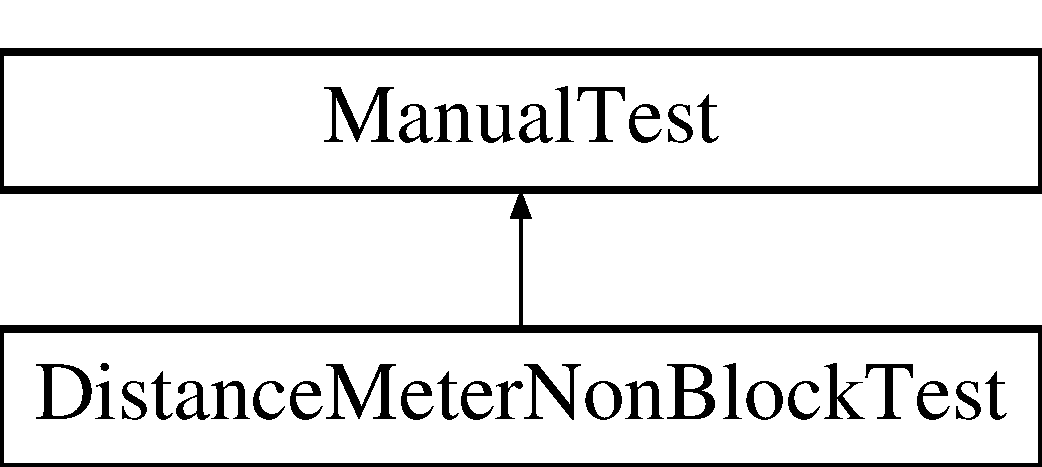
\includegraphics[height=2.000000cm]{class_distance_meter_non_block_test}
\end{center}
\end{figure}
\subsection*{Public Member Functions}
\begin{DoxyCompactItemize}
\item 
\mbox{\Hypertarget{class_distance_meter_non_block_test_a99e42bd9c7d0238c003e061cfcf56cfa}\label{class_distance_meter_non_block_test_a99e42bd9c7d0238c003e061cfcf56cfa}} 
{\bfseries Distance\+Meter\+Non\+Block\+Test} (Stream \&debug\+Stream, uint8\+\_\+t trigger\+Pin, uint8\+\_\+t echo\+Pin)
\end{DoxyCompactItemize}
\subsection*{Protected Member Functions}
\begin{DoxyCompactItemize}
\item 
\mbox{\Hypertarget{class_distance_meter_non_block_test_a183198c75523b1713a520222cfe234fe}\label{class_distance_meter_non_block_test_a183198c75523b1713a520222cfe234fe}} 
void {\bfseries tests\+Setup} ()
\item 
\mbox{\Hypertarget{class_distance_meter_non_block_test_adbda1a19bc7753473f52d5eb37f8b35e}\label{class_distance_meter_non_block_test_adbda1a19bc7753473f52d5eb37f8b35e}} 
void {\bfseries tests} ()
\item 
\mbox{\Hypertarget{class_distance_meter_non_block_test_aba1fc21d6c1f087c224a9269d76eb5a8}\label{class_distance_meter_non_block_test_aba1fc21d6c1f087c224a9269d76eb5a8}} 
void {\bfseries after\+Test\+Suite} ()
\end{DoxyCompactItemize}
\subsection*{Additional Inherited Members}


The documentation for this class was generated from the following file\+:\begin{DoxyCompactItemize}
\item 
src/tests/Distance\+Meter\+Non\+Block\+Test.\+h\end{DoxyCompactItemize}

\hypertarget{class_easyuino_1_1_distance_meter_printable}{}\section{Easyuino\+:\+:Distance\+Meter\+Printable Class Reference}
\label{class_easyuino_1_1_distance_meter_printable}\index{Easyuino\+::\+Distance\+Meter\+Printable@{Easyuino\+::\+Distance\+Meter\+Printable}}
Inheritance diagram for Easyuino\+:\+:Distance\+Meter\+Printable\+:\begin{figure}[H]
\begin{center}
\leavevmode
\includegraphics[height=3.000000cm]{class_easyuino_1_1_distance_meter_printable}
\end{center}
\end{figure}
\subsection*{Public Member Functions}
\begin{DoxyCompactItemize}
\item 
\mbox{\Hypertarget{class_easyuino_1_1_distance_meter_printable_a367fe13996801c142f687234390bfc8c}\label{class_easyuino_1_1_distance_meter_printable_a367fe13996801c142f687234390bfc8c}} 
{\bfseries Distance\+Meter\+Printable} (IN uint8\+\_\+t trigger\+Pin, IN uint8\+\_\+t echo\+Pin)
\item 
\mbox{\Hypertarget{class_easyuino_1_1_distance_meter_printable_a4a7366a8f46038026a0b5023826da83f}\label{class_easyuino_1_1_distance_meter_printable_a4a7366a8f46038026a0b5023826da83f}} 
char $\ast$ {\bfseries to\+String} () const
\end{DoxyCompactItemize}
\subsection*{Additional Inherited Members}


The documentation for this class was generated from the following files\+:\begin{DoxyCompactItemize}
\item 
src/Distance\+Meter\+Printable.\+h\item 
src/main/\+Ultrasonic/Distance\+Meter\+Printable.\+cpp\end{DoxyCompactItemize}

\hypertarget{class_distance_meter_test}{}\section{Distance\+Meter\+Test Class Reference}
\label{class_distance_meter_test}\index{Distance\+Meter\+Test@{Distance\+Meter\+Test}}
Inheritance diagram for Distance\+Meter\+Test\+:\begin{figure}[H]
\begin{center}
\leavevmode
\includegraphics[height=2.000000cm]{class_distance_meter_test}
\end{center}
\end{figure}
\subsection*{Public Member Functions}
\begin{DoxyCompactItemize}
\item 
\mbox{\Hypertarget{class_distance_meter_test_a72bec787e1e981840ea0399d68a18ac1}\label{class_distance_meter_test_a72bec787e1e981840ea0399d68a18ac1}} 
{\bfseries Distance\+Meter\+Test} (Stream \&debug\+Stream, uint8\+\_\+t trigger\+Pin, uint8\+\_\+t echo\+Pin)
\end{DoxyCompactItemize}
\subsection*{Protected Member Functions}
\begin{DoxyCompactItemize}
\item 
\mbox{\Hypertarget{class_distance_meter_test_a3e9d2311b2c2740515cf70d904b20271}\label{class_distance_meter_test_a3e9d2311b2c2740515cf70d904b20271}} 
void {\bfseries tests\+Setup} ()
\item 
\mbox{\Hypertarget{class_distance_meter_test_ac82e881bf404ac3b9b8c16c997f8e39e}\label{class_distance_meter_test_ac82e881bf404ac3b9b8c16c997f8e39e}} 
void {\bfseries tests} ()
\item 
\mbox{\Hypertarget{class_distance_meter_test_ad3b3e352542cf2f1130e73bdc7d440b7}\label{class_distance_meter_test_ad3b3e352542cf2f1130e73bdc7d440b7}} 
void {\bfseries after\+Test\+Suite} ()
\end{DoxyCompactItemize}
\subsection*{Additional Inherited Members}


The documentation for this class was generated from the following file\+:\begin{DoxyCompactItemize}
\item 
src/tests/Distance\+Meter\+Test.\+h\end{DoxyCompactItemize}

\hypertarget{class_easyuino_1_1_g_s_m_service}{}\section{Easyuino\+:\+:G\+S\+M\+Service Class Reference}
\label{class_easyuino_1_1_g_s_m_service}\index{Easyuino\+::\+G\+S\+M\+Service@{Easyuino\+::\+G\+S\+M\+Service}}
Inheritance diagram for Easyuino\+:\+:G\+S\+M\+Service\+:\begin{figure}[H]
\begin{center}
\leavevmode
\includegraphics[height=3.000000cm]{class_easyuino_1_1_g_s_m_service}
\end{center}
\end{figure}
\subsection*{Public Member Functions}
\begin{DoxyCompactItemize}
\item 
\mbox{\Hypertarget{class_easyuino_1_1_g_s_m_service_ad8700c921a8f3ce267369e9843853be1}\label{class_easyuino_1_1_g_s_m_service_ad8700c921a8f3ce267369e9843853be1}} 
{\bfseries G\+S\+M\+Service} (IN uint8\+\_\+t tx\+Pin, IN uint8\+\_\+t rx\+Pin, IN uint8\+\_\+t power\+Pin, IN Stream \&output\+Stream)
\item 
\mbox{\Hypertarget{class_easyuino_1_1_g_s_m_service_ab856f1ecdb47de6b13f186bea7c69ce2}\label{class_easyuino_1_1_g_s_m_service_ab856f1ecdb47de6b13f186bea7c69ce2}} 
{\bfseries G\+S\+M\+Service} (IN uint8\+\_\+t tx\+Pin, IN uint8\+\_\+t rx\+Pin, IN uint8\+\_\+t power\+Pin)
\item 
\mbox{\Hypertarget{class_easyuino_1_1_g_s_m_service_a49dd695dba030b168464f620c3d96ee0}\label{class_easyuino_1_1_g_s_m_service_a49dd695dba030b168464f620c3d96ee0}} 
bool {\bfseries begin} (IN unsigned long gsm\+Module\+Baud\+Rate)
\item 
bool \hyperlink{class_easyuino_1_1_g_s_m_service_aeafc2dae47e4b13e127eb228a0f7ff6a}{begin} ()
\begin{DoxyCompactList}\small\item\em Used to put the device ready to receive requests. \end{DoxyCompactList}\item 
void \hyperlink{class_easyuino_1_1_g_s_m_service_a05bef783773776ec209608aa81d1ff45}{end} ()
\begin{DoxyCompactList}\small\item\em Used to stop the device A\+PI. \end{DoxyCompactList}\item 
\mbox{\Hypertarget{class_easyuino_1_1_g_s_m_service_ad5bd54c7dfcc402df0fac92c88e07c6e}\label{class_easyuino_1_1_g_s_m_service_ad5bd54c7dfcc402df0fac92c88e07c6e}} 
G\+S\+M\+Request\+Status {\bfseries turn\+On} ()
\item 
\mbox{\Hypertarget{class_easyuino_1_1_g_s_m_service_a327c2610c2aa7ba5a54530d87a0d6128}\label{class_easyuino_1_1_g_s_m_service_a327c2610c2aa7ba5a54530d87a0d6128}} 
G\+S\+M\+Request\+Status {\bfseries turn\+Off} ()
\item 
\mbox{\Hypertarget{class_easyuino_1_1_g_s_m_service_a2ad440efbd04942d956212988d20a0df}\label{class_easyuino_1_1_g_s_m_service_a2ad440efbd04942d956212988d20a0df}} 
G\+S\+M\+Request\+Status {\bfseries is\+On} (O\+UT bool \&result)
\item 
\mbox{\Hypertarget{class_easyuino_1_1_g_s_m_service_a6b6ee723ceaf62bfd9312278b5dbf36d}\label{class_easyuino_1_1_g_s_m_service_a6b6ee723ceaf62bfd9312278b5dbf36d}} 
G\+S\+M\+Request\+Status {\bfseries set\+Baud\+Rate} (IN unsigned long new\+Baud\+Rate)
\item 
\mbox{\Hypertarget{class_easyuino_1_1_g_s_m_service_a8fd764ef215a16f676e6e5e4b283b61d}\label{class_easyuino_1_1_g_s_m_service_a8fd764ef215a16f676e6e5e4b283b61d}} 
G\+S\+M\+Request\+Status {\bfseries begin\+Listen\+For\+S\+MS} ()
\item 
\mbox{\Hypertarget{class_easyuino_1_1_g_s_m_service_a02c2bddace1c87f035f324ae248c4f1d}\label{class_easyuino_1_1_g_s_m_service_a02c2bddace1c87f035f324ae248c4f1d}} 
virtual G\+S\+M\+Request\+Status {\bfseries available\+S\+MS} (O\+UT \hyperlink{class_easyuino_1_1_s_m_s}{S\+MS} \&message, O\+UT bool \&sms\+Read)
\item 
\mbox{\Hypertarget{class_easyuino_1_1_g_s_m_service_ae860cc330ef552c733d9ab4a5c2fd366}\label{class_easyuino_1_1_g_s_m_service_ae860cc330ef552c733d9ab4a5c2fd366}} 
G\+S\+M\+Request\+Status {\bfseries send\+S\+MS} (IN \hyperlink{class_easyuino_1_1_s_m_s}{S\+MS} \&sms)
\item 
\mbox{\Hypertarget{class_easyuino_1_1_g_s_m_service_ad37d83f2a91fbe2e50a11f1d435eccb5}\label{class_easyuino_1_1_g_s_m_service_ad37d83f2a91fbe2e50a11f1d435eccb5}} 
G\+S\+M\+Request\+Status {\bfseries send\+S\+MS} (IN unsigned long phone\+Number, IN const char $\ast$message, IN unsigned int country\+Prefix\+Code)
\item 
\mbox{\Hypertarget{class_easyuino_1_1_g_s_m_service_aef4379e7c82f275f0af341f79a3b451f}\label{class_easyuino_1_1_g_s_m_service_aef4379e7c82f275f0af341f79a3b451f}} 
G\+S\+M\+Request\+Status {\bfseries delete\+All\+S\+MS} ()
\item 
\mbox{\Hypertarget{class_easyuino_1_1_g_s_m_service_af142e4f7d99cffda9a3598446466cdb3}\label{class_easyuino_1_1_g_s_m_service_af142e4f7d99cffda9a3598446466cdb3}} 
G\+S\+M\+Request\+Status {\bfseries delete\+All\+Read\+S\+MS} ()
\item 
\mbox{\Hypertarget{class_easyuino_1_1_g_s_m_service_a7b457ab0669a8e9c16ab1906cc246365}\label{class_easyuino_1_1_g_s_m_service_a7b457ab0669a8e9c16ab1906cc246365}} 
G\+S\+M\+Request\+Status {\bfseries delete\+All\+Sent\+And\+Read\+S\+MS} ()
\end{DoxyCompactItemize}
\subsection*{Additional Inherited Members}


\subsection{Member Function Documentation}
\mbox{\Hypertarget{class_easyuino_1_1_g_s_m_service_aeafc2dae47e4b13e127eb228a0f7ff6a}\label{class_easyuino_1_1_g_s_m_service_aeafc2dae47e4b13e127eb228a0f7ff6a}} 
\index{Easyuino\+::\+G\+S\+M\+Service@{Easyuino\+::\+G\+S\+M\+Service}!begin@{begin}}
\index{begin@{begin}!Easyuino\+::\+G\+S\+M\+Service@{Easyuino\+::\+G\+S\+M\+Service}}
\subsubsection{\texorpdfstring{begin()}{begin()}}
{\footnotesize\ttfamily bool Easyuino\+::\+G\+S\+M\+Service\+::begin (\begin{DoxyParamCaption}{ }\end{DoxyParamCaption})\hspace{0.3cm}{\ttfamily [virtual]}}



Used to put the device ready to receive requests. 

Normally this have some default behaviour some devices have other overload method with same name that receives other arguments to device customization. \begin{DoxyReturn}{Returns}
True\+: If the device was initialized. False\+: Otherwise. 
\end{DoxyReturn}


Implements \hyperlink{class_easyuino_1_1_device_a2e7bb2fec849719a9d9432b57cdb72ba}{Easyuino\+::\+Device}.

\mbox{\Hypertarget{class_easyuino_1_1_g_s_m_service_a05bef783773776ec209608aa81d1ff45}\label{class_easyuino_1_1_g_s_m_service_a05bef783773776ec209608aa81d1ff45}} 
\index{Easyuino\+::\+G\+S\+M\+Service@{Easyuino\+::\+G\+S\+M\+Service}!end@{end}}
\index{end@{end}!Easyuino\+::\+G\+S\+M\+Service@{Easyuino\+::\+G\+S\+M\+Service}}
\subsubsection{\texorpdfstring{end()}{end()}}
{\footnotesize\ttfamily void Easyuino\+::\+G\+S\+M\+Service\+::end (\begin{DoxyParamCaption}{ }\end{DoxyParamCaption})\hspace{0.3cm}{\ttfamily [virtual]}}



Used to stop the device A\+PI. 

After this the the device will not process A\+PI requests. 

Implements \hyperlink{class_easyuino_1_1_device_ab31018ef64adc84aa2ea575b2297548f}{Easyuino\+::\+Device}.



The documentation for this class was generated from the following file\+:\begin{DoxyCompactItemize}
\item 
src/G\+S\+M\+Service.\+h\end{DoxyCompactItemize}

\hypertarget{class_easyuino_1_1_g_s_m_service_secure}{}\section{Easyuino\+:\+:G\+S\+M\+Service\+Secure Class Reference}
\label{class_easyuino_1_1_g_s_m_service_secure}\index{Easyuino\+::\+G\+S\+M\+Service\+Secure@{Easyuino\+::\+G\+S\+M\+Service\+Secure}}
Inheritance diagram for Easyuino\+:\+:G\+S\+M\+Service\+Secure\+:\begin{figure}[H]
\begin{center}
\leavevmode
\includegraphics[height=3.000000cm]{class_easyuino_1_1_g_s_m_service_secure}
\end{center}
\end{figure}
\subsection*{Public Member Functions}
\begin{DoxyCompactItemize}
\item 
\mbox{\Hypertarget{class_easyuino_1_1_g_s_m_service_secure_ab28bad6e7765f61851a3957edc5d3071}\label{class_easyuino_1_1_g_s_m_service_secure_ab28bad6e7765f61851a3957edc5d3071}} 
{\bfseries G\+S\+M\+Service\+Secure} (IN uint8\+\_\+t tx\+Pin, IN uint8\+\_\+t rx\+Pin, IN uint8\+\_\+t power\+Pin, IN Stream \&output\+Stream)
\item 
\mbox{\Hypertarget{class_easyuino_1_1_g_s_m_service_secure_a4331122e2c6e42711eb13bf59cfd940c}\label{class_easyuino_1_1_g_s_m_service_secure_a4331122e2c6e42711eb13bf59cfd940c}} 
{\bfseries G\+S\+M\+Service\+Secure} (IN uint8\+\_\+t tx\+Pin, IN uint8\+\_\+t rx\+Pin, IN uint8\+\_\+t power\+Pin)
\item 
\mbox{\Hypertarget{class_easyuino_1_1_g_s_m_service_secure_a7acbf1d460ef1b81bcd36d852b596af3}\label{class_easyuino_1_1_g_s_m_service_secure_a7acbf1d460ef1b81bcd36d852b596af3}} 
G\+S\+M\+Request\+Status {\bfseries add\+Allowed\+Number} (IN unsigned long phone\+Number\+To\+Add)
\item 
\mbox{\Hypertarget{class_easyuino_1_1_g_s_m_service_secure_a791dd872fe2c72311d84219616e5f54c}\label{class_easyuino_1_1_g_s_m_service_secure_a791dd872fe2c72311d84219616e5f54c}} 
G\+S\+M\+Request\+Status {\bfseries is\+Allowed} (IN unsigned long phone\+Number, O\+UT bool \&allowed)
\item 
\mbox{\Hypertarget{class_easyuino_1_1_g_s_m_service_secure_a1ad4988fa2dcc0ba8f87c70cf71edf29}\label{class_easyuino_1_1_g_s_m_service_secure_a1ad4988fa2dcc0ba8f87c70cf71edf29}} 
G\+S\+M\+Request\+Status {\bfseries remove\+Allowed\+Number} (IN unsigned long phone\+Number\+To\+Remove)
\item 
\mbox{\Hypertarget{class_easyuino_1_1_g_s_m_service_secure_a10a8160dfb473d84b4bd182d689bdb95}\label{class_easyuino_1_1_g_s_m_service_secure_a10a8160dfb473d84b4bd182d689bdb95}} 
G\+S\+M\+Request\+Status {\bfseries clear\+Allowed\+Numbers} ()
\item 
\mbox{\Hypertarget{class_easyuino_1_1_g_s_m_service_secure_acd045866feff695131d00d7bdd9def0a}\label{class_easyuino_1_1_g_s_m_service_secure_acd045866feff695131d00d7bdd9def0a}} 
virtual G\+S\+M\+Request\+Status {\bfseries available\+S\+MS} (I\+N\+O\+UT \hyperlink{class_easyuino_1_1_s_m_s}{S\+MS} \&message, O\+UT bool \&sms\+Read)
\end{DoxyCompactItemize}
\subsection*{Additional Inherited Members}


The documentation for this class was generated from the following files\+:\begin{DoxyCompactItemize}
\item 
src/G\+S\+M\+Service\+Secure.\+h\item 
src/main/\+G\+S\+M/G\+S\+M\+Service\+Secure.\+cpp\end{DoxyCompactItemize}

\hypertarget{class_easyuino_1_1_infra_red_receiver}{}\section{Easyuino\+:\+:Infra\+Red\+Receiver Class Reference}
\label{class_easyuino_1_1_infra_red_receiver}\index{Easyuino\+::\+Infra\+Red\+Receiver@{Easyuino\+::\+Infra\+Red\+Receiver}}
Inheritance diagram for Easyuino\+:\+:Infra\+Red\+Receiver\+:\begin{figure}[H]
\begin{center}
\leavevmode
\includegraphics[height=2.000000cm]{class_easyuino_1_1_infra_red_receiver}
\end{center}
\end{figure}
\subsection*{Additional Inherited Members}


The documentation for this class was generated from the following file\+:\begin{DoxyCompactItemize}
\item 
src/Infra\+Red\+Receiver.\+h\end{DoxyCompactItemize}

\hypertarget{class_manual_test}{}\section{Manual\+Test Class Reference}
\label{class_manual_test}\index{Manual\+Test@{Manual\+Test}}
Inheritance diagram for Manual\+Test\+:\begin{figure}[H]
\begin{center}
\leavevmode
\includegraphics[height=0.893855cm]{class_manual_test}
\end{center}
\end{figure}
\subsection*{Public Member Functions}
\begin{DoxyCompactItemize}
\item 
\mbox{\Hypertarget{class_manual_test_aceabb8c03fd5d4f40310ed58d52f519f}\label{class_manual_test_aceabb8c03fd5d4f40310ed58d52f519f}} 
{\bfseries Manual\+Test} (Stream \&debug\+Stream)
\item 
\mbox{\Hypertarget{class_manual_test_afdebad9843c466bcccbf74f9bc3390e6}\label{class_manual_test_afdebad9843c466bcccbf74f9bc3390e6}} 
void {\bfseries run\+Tests\+Setup} ()
\item 
\mbox{\Hypertarget{class_manual_test_a6d8ca4fbf873f18d9602353d41241aae}\label{class_manual_test_a6d8ca4fbf873f18d9602353d41241aae}} 
void {\bfseries run\+Tests} ()
\end{DoxyCompactItemize}
\subsection*{Protected Member Functions}
\begin{DoxyCompactItemize}
\item 
\mbox{\Hypertarget{class_manual_test_ab3c40aab099320672b7524b84582fef1}\label{class_manual_test_ab3c40aab099320672b7524b84582fef1}} 
virtual void {\bfseries tests\+Setup} ()=0
\item 
\mbox{\Hypertarget{class_manual_test_a34284ba4f0d9cf915bee6d3f18adab82}\label{class_manual_test_a34284ba4f0d9cf915bee6d3f18adab82}} 
virtual void {\bfseries tests} ()=0
\item 
\mbox{\Hypertarget{class_manual_test_a20134c6b27c5f09e92c6957b0cb2fc8b}\label{class_manual_test_a20134c6b27c5f09e92c6957b0cb2fc8b}} 
virtual void {\bfseries before\+Test} ()
\item 
\mbox{\Hypertarget{class_manual_test_a9450c75b9bbbab5540195f216a61449e}\label{class_manual_test_a9450c75b9bbbab5540195f216a61449e}} 
virtual void {\bfseries after\+Test} ()
\item 
\mbox{\Hypertarget{class_manual_test_a7bade8194573f592eb16503de3017d86}\label{class_manual_test_a7bade8194573f592eb16503de3017d86}} 
virtual void {\bfseries after\+Test\+Suite} ()
\item 
\mbox{\Hypertarget{class_manual_test_ab66c12b2cecf1e09532a8da12e97b036}\label{class_manual_test_ab66c12b2cecf1e09532a8da12e97b036}} 
void {\bfseries test\+Start} (char $\ast$str)
\item 
\mbox{\Hypertarget{class_manual_test_a1ea97c89dcceb0e686c9973eda31ed1a}\label{class_manual_test_a1ea97c89dcceb0e686c9973eda31ed1a}} 
void {\bfseries test\+End} (unsigned long delay\+After\+Test\+Override=D\+E\+L\+A\+Y\+\_\+\+B\+E\+T\+W\+E\+E\+N\+\_\+\+T\+E\+S\+TS)
\end{DoxyCompactItemize}
\subsection*{Protected Attributes}
\begin{DoxyCompactItemize}
\item 
\mbox{\Hypertarget{class_manual_test_afc47b14a8b3427b999b63451aee90f4e}\label{class_manual_test_afc47b14a8b3427b999b63451aee90f4e}} 
Stream $\ast$ {\bfseries \+\_\+debug\+Stream}
\end{DoxyCompactItemize}


The documentation for this class was generated from the following files\+:\begin{DoxyCompactItemize}
\item 
src/tests/Manual\+Test.\+h\item 
src/tests/Manual\+Test.\+cpp\end{DoxyCompactItemize}

\hypertarget{class_easyuino_1_1_printable}{}\section{Easyuino\+:\+:Printable Class Reference}
\label{class_easyuino_1_1_printable}\index{Easyuino\+::\+Printable@{Easyuino\+::\+Printable}}
Inheritance diagram for Easyuino\+:\+:Printable\+:\begin{figure}[H]
\begin{center}
\leavevmode
\includegraphics[height=2.000000cm]{class_easyuino_1_1_printable}
\end{center}
\end{figure}
\subsection*{Public Member Functions}
\begin{DoxyCompactItemize}
\item 
\mbox{\Hypertarget{class_easyuino_1_1_printable_a49ae1c60dc0404600ee122c6c2684155}\label{class_easyuino_1_1_printable_a49ae1c60dc0404600ee122c6c2684155}} 
virtual char $\ast$ {\bfseries to\+String} () const =0
\end{DoxyCompactItemize}
\subsection*{Friends}
\begin{DoxyCompactItemize}
\item 
\mbox{\Hypertarget{class_easyuino_1_1_printable_a50c7f93c6a84fde9f1f97f1185d853d9}\label{class_easyuino_1_1_printable_a50c7f93c6a84fde9f1f97f1185d853d9}} 
Stream \& {\bfseries operator$<$$<$} (IN Stream \&stream, IN const \hyperlink{class_easyuino_1_1_printable}{Printable} \&printable)
\end{DoxyCompactItemize}


The documentation for this class was generated from the following file\+:\begin{DoxyCompactItemize}
\item 
src/Printable.\+h\end{DoxyCompactItemize}

\hypertarget{class_easyuino_1_1_relay}{}\section{Easyuino\+:\+:Relay Class Reference}
\label{class_easyuino_1_1_relay}\index{Easyuino\+::\+Relay@{Easyuino\+::\+Relay}}
Inheritance diagram for Easyuino\+:\+:Relay\+:\begin{figure}[H]
\begin{center}
\leavevmode
\includegraphics[height=3.000000cm]{class_easyuino_1_1_relay}
\end{center}
\end{figure}
\subsection*{Public Member Functions}
\begin{DoxyCompactItemize}
\item 
\mbox{\Hypertarget{class_easyuino_1_1_relay_a34a9e8461a4018e88ee49d956aca37f7}\label{class_easyuino_1_1_relay_a34a9e8461a4018e88ee49d956aca37f7}} 
{\bfseries Relay} (IN uint8\+\_\+t arduino\+Pin)
\item 
bool \hyperlink{class_easyuino_1_1_relay_a920a0fa287cacfd8c6df19d8812d4958}{begin} ()
\begin{DoxyCompactList}\small\item\em Used to put the device ready to receive requests. \end{DoxyCompactList}\item 
\mbox{\Hypertarget{class_easyuino_1_1_relay_a05e66468ee1b991f394d9182b9886bf7}\label{class_easyuino_1_1_relay_a05e66468ee1b991f394d9182b9886bf7}} 
bool {\bfseries begin} (IN bool is\+Normally\+Closed, IN uint8\+\_\+t normally\+Closed\+Pin\+Level)
\item 
void \hyperlink{class_easyuino_1_1_relay_a2b57237c996a6ffe8e900ae273bce9d4}{end} ()
\begin{DoxyCompactList}\small\item\em Used to stop the device A\+PI. \end{DoxyCompactList}\item 
\mbox{\Hypertarget{class_easyuino_1_1_relay_a28b594b3ee957e062630fa2c771a966d}\label{class_easyuino_1_1_relay_a28b594b3ee957e062630fa2c771a966d}} 
void {\bfseries turn\+On} ()
\item 
\mbox{\Hypertarget{class_easyuino_1_1_relay_a9cab51ad0aaea32752df829f3f6b8113}\label{class_easyuino_1_1_relay_a9cab51ad0aaea32752df829f3f6b8113}} 
void {\bfseries turn\+Off} ()
\item 
\mbox{\Hypertarget{class_easyuino_1_1_relay_af8b4ac99e27ffac6c5f8d69d36dc01f5}\label{class_easyuino_1_1_relay_af8b4ac99e27ffac6c5f8d69d36dc01f5}} 
bool {\bfseries is\+On} () const
\end{DoxyCompactItemize}
\subsection*{Additional Inherited Members}


\subsection{Member Function Documentation}
\mbox{\Hypertarget{class_easyuino_1_1_relay_a920a0fa287cacfd8c6df19d8812d4958}\label{class_easyuino_1_1_relay_a920a0fa287cacfd8c6df19d8812d4958}} 
\index{Easyuino\+::\+Relay@{Easyuino\+::\+Relay}!begin@{begin}}
\index{begin@{begin}!Easyuino\+::\+Relay@{Easyuino\+::\+Relay}}
\subsubsection{\texorpdfstring{begin()}{begin()}}
{\footnotesize\ttfamily bool Easyuino\+::\+Relay\+::begin (\begin{DoxyParamCaption}{ }\end{DoxyParamCaption})\hspace{0.3cm}{\ttfamily [virtual]}}



Used to put the device ready to receive requests. 

Normally this have some default behaviour some devices have other overload method with same name that receives other arguments to device customization. \begin{DoxyReturn}{Returns}
True\+: If the device was initialized. False\+: Otherwise. 
\end{DoxyReturn}


Implements \hyperlink{class_easyuino_1_1_device_a2e7bb2fec849719a9d9432b57cdb72ba}{Easyuino\+::\+Device}.

\mbox{\Hypertarget{class_easyuino_1_1_relay_a2b57237c996a6ffe8e900ae273bce9d4}\label{class_easyuino_1_1_relay_a2b57237c996a6ffe8e900ae273bce9d4}} 
\index{Easyuino\+::\+Relay@{Easyuino\+::\+Relay}!end@{end}}
\index{end@{end}!Easyuino\+::\+Relay@{Easyuino\+::\+Relay}}
\subsubsection{\texorpdfstring{end()}{end()}}
{\footnotesize\ttfamily void Easyuino\+::\+Relay\+::end (\begin{DoxyParamCaption}{ }\end{DoxyParamCaption})\hspace{0.3cm}{\ttfamily [virtual]}}



Used to stop the device A\+PI. 

After this the the device will not process A\+PI requests. 

Implements \hyperlink{class_easyuino_1_1_device_ab31018ef64adc84aa2ea575b2297548f}{Easyuino\+::\+Device}.



The documentation for this class was generated from the following file\+:\begin{DoxyCompactItemize}
\item 
src/Relay.\+h\end{DoxyCompactItemize}

\hypertarget{class_easyuino_1_1_relay_named}{}\section{Easyuino\+:\+:Relay\+Named Class Reference}
\label{class_easyuino_1_1_relay_named}\index{Easyuino\+::\+Relay\+Named@{Easyuino\+::\+Relay\+Named}}


\hyperlink{class_easyuino_1_1_relay_named}{Relay\+Named} offers the same A\+PI of the \hyperlink{class_easyuino_1_1_relay}{Relay} plus the possibility to associate a string label to the A\+PI object.  




{\ttfamily \#include $<$Relay\+Named.\+h$>$}

Inheritance diagram for Easyuino\+:\+:Relay\+Named\+:\begin{figure}[H]
\begin{center}
\leavevmode
\includegraphics[height=3.000000cm]{class_easyuino_1_1_relay_named}
\end{center}
\end{figure}
\subsection*{Public Member Functions}
\begin{DoxyCompactItemize}
\item 
\hyperlink{class_easyuino_1_1_relay_named_a3def4eb321085beb48fa3e45da5e6dfc}{Relay\+Named} (IN uint8\+\_\+t arduino\+Pin, IN const char $\ast$device\+Name)
\begin{DoxyCompactList}\small\item\em Constructor. \end{DoxyCompactList}\item 
char $\ast$ \hyperlink{class_easyuino_1_1_relay_named_a1e9e82e563baaba5055ee9335551a306}{to\+String} () const
\begin{DoxyCompactList}\small\item\em Used to return a string representation of the object state. \end{DoxyCompactList}\end{DoxyCompactItemize}
\subsection*{Additional Inherited Members}


\subsection{Detailed Description}
\hyperlink{class_easyuino_1_1_relay_named}{Relay\+Named} offers the same A\+PI of the \hyperlink{class_easyuino_1_1_relay}{Relay} plus the possibility to associate a string label to the A\+PI object. 

\begin{DoxySeeAlso}{See also}
Devices Supported\+: S\+R\+D-\/05\+V\+D\+C-\/\+S\+L-\/C, Probably any relay because they are very simple devices 

Devices Tested\+: S\+R\+D-\/05\+V\+D\+C-\/\+S\+L-\/C 
\end{DoxySeeAlso}


\subsection{Constructor \& Destructor Documentation}
\mbox{\Hypertarget{class_easyuino_1_1_relay_named_a3def4eb321085beb48fa3e45da5e6dfc}\label{class_easyuino_1_1_relay_named_a3def4eb321085beb48fa3e45da5e6dfc}} 
\index{Easyuino\+::\+Relay\+Named@{Easyuino\+::\+Relay\+Named}!Relay\+Named@{Relay\+Named}}
\index{Relay\+Named@{Relay\+Named}!Easyuino\+::\+Relay\+Named@{Easyuino\+::\+Relay\+Named}}
\subsubsection{\texorpdfstring{Relay\+Named()}{RelayNamed()}}
{\footnotesize\ttfamily Easyuino\+::\+Relay\+Named\+::\+Relay\+Named (\begin{DoxyParamCaption}\item[{IN uint8\+\_\+t}]{arduino\+Pin,  }\item[{IN const char $\ast$}]{device\+Name }\end{DoxyParamCaption})}



Constructor. 


\begin{DoxyParams}{Parameters}
{\em arduino\+Pin} & Arduino pin that is connected with the relay (normal in relay is IN pins) \\
\hline
{\em device\+Name} & Name (identifier) of the device that the relay activates/deactivates \\
\hline
\end{DoxyParams}


\subsection{Member Function Documentation}
\mbox{\Hypertarget{class_easyuino_1_1_relay_named_a1e9e82e563baaba5055ee9335551a306}\label{class_easyuino_1_1_relay_named_a1e9e82e563baaba5055ee9335551a306}} 
\index{Easyuino\+::\+Relay\+Named@{Easyuino\+::\+Relay\+Named}!to\+String@{to\+String}}
\index{to\+String@{to\+String}!Easyuino\+::\+Relay\+Named@{Easyuino\+::\+Relay\+Named}}
\subsubsection{\texorpdfstring{to\+String()}{toString()}}
{\footnotesize\ttfamily char$\ast$ Easyuino\+::\+Relay\+Named\+::to\+String (\begin{DoxyParamCaption}{ }\end{DoxyParamCaption}) const\hspace{0.3cm}{\ttfamily [virtual]}}



Used to return a string representation of the object state. 

I\+M\+P\+O\+R\+T\+A\+NT\+: It is mandatory to free the returned pointer in order to have no memory leaks. 

Implements \hyperlink{class_easyuino_1_1_printable_a49ae1c60dc0404600ee122c6c2684155}{Easyuino\+::\+Printable}.



The documentation for this class was generated from the following file\+:\begin{DoxyCompactItemize}
\item 
src/Relay\+Named.\+h\end{DoxyCompactItemize}

\hypertarget{class_relay_named_test}{}\section{Relay\+Named\+Test Class Reference}
\label{class_relay_named_test}\index{Relay\+Named\+Test@{Relay\+Named\+Test}}
Inheritance diagram for Relay\+Named\+Test\+:\begin{figure}[H]
\begin{center}
\leavevmode
\includegraphics[height=2.000000cm]{class_relay_named_test}
\end{center}
\end{figure}
\subsection*{Public Member Functions}
\begin{DoxyCompactItemize}
\item 
\mbox{\Hypertarget{class_relay_named_test_a6d38b8013435f4ac48c69ea7453491d3}\label{class_relay_named_test_a6d38b8013435f4ac48c69ea7453491d3}} 
{\bfseries Relay\+Named\+Test} (Stream \&debug\+Stream, uint8\+\_\+t arduino\+Pin, const char $\ast$relay\+Name)
\end{DoxyCompactItemize}
\subsection*{Protected Member Functions}
\begin{DoxyCompactItemize}
\item 
\mbox{\Hypertarget{class_relay_named_test_a40838e4025039d18b1d05f2d6d9613e8}\label{class_relay_named_test_a40838e4025039d18b1d05f2d6d9613e8}} 
void {\bfseries tests\+Setup} ()
\item 
\mbox{\Hypertarget{class_relay_named_test_af4b0f4ec6ba0f8e1434221dfc401c823}\label{class_relay_named_test_af4b0f4ec6ba0f8e1434221dfc401c823}} 
void {\bfseries tests} ()
\item 
\mbox{\Hypertarget{class_relay_named_test_af44928bffbb1d2733f12569dff36e3a1}\label{class_relay_named_test_af44928bffbb1d2733f12569dff36e3a1}} 
void {\bfseries after\+Test\+Suite} ()
\end{DoxyCompactItemize}
\subsection*{Additional Inherited Members}


The documentation for this class was generated from the following file\+:\begin{DoxyCompactItemize}
\item 
src/tests/Relay\+Named\+Test.\+h\end{DoxyCompactItemize}

\hypertarget{class_relay_test}{}\section{Relay\+Test Class Reference}
\label{class_relay_test}\index{Relay\+Test@{Relay\+Test}}
Inheritance diagram for Relay\+Test\+:\begin{figure}[H]
\begin{center}
\leavevmode
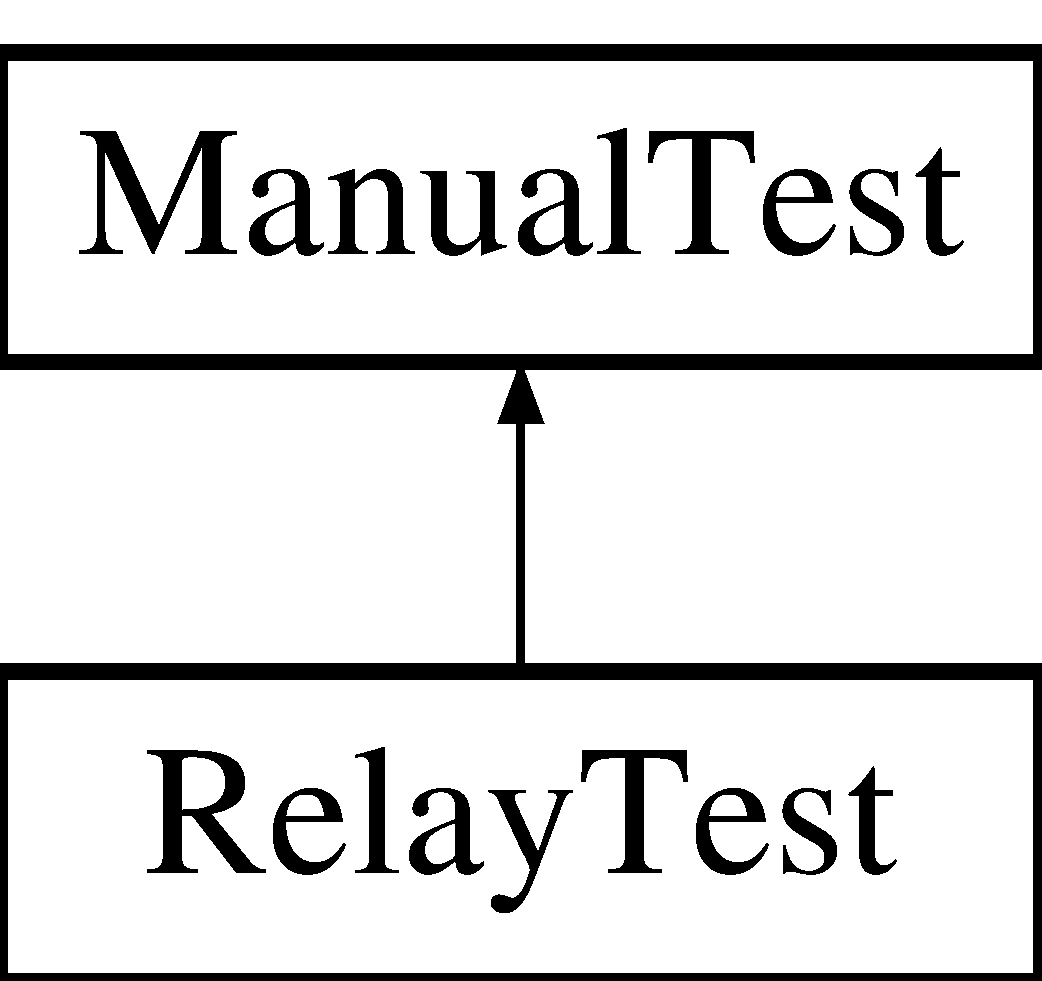
\includegraphics[height=2.000000cm]{class_relay_test}
\end{center}
\end{figure}
\subsection*{Public Member Functions}
\begin{DoxyCompactItemize}
\item 
\mbox{\Hypertarget{class_relay_test_abaee9a70df57128ba571b69fc784c258}\label{class_relay_test_abaee9a70df57128ba571b69fc784c258}} 
{\bfseries Relay\+Test} (Stream \&debug\+Stream, uint8\+\_\+t arduino\+Pin)
\end{DoxyCompactItemize}
\subsection*{Protected Member Functions}
\begin{DoxyCompactItemize}
\item 
\mbox{\Hypertarget{class_relay_test_a1644f898816a9c6cf57e6cc1c73bdc24}\label{class_relay_test_a1644f898816a9c6cf57e6cc1c73bdc24}} 
void {\bfseries tests\+Setup} ()
\item 
\mbox{\Hypertarget{class_relay_test_a15a64ece66ce3f6a9ea09101d744e73b}\label{class_relay_test_a15a64ece66ce3f6a9ea09101d744e73b}} 
void {\bfseries tests} ()
\item 
\mbox{\Hypertarget{class_relay_test_aaa61a82f1eb59f1b93085478f029c741}\label{class_relay_test_aaa61a82f1eb59f1b93085478f029c741}} 
void {\bfseries after\+Test\+Suite} ()
\end{DoxyCompactItemize}
\subsection*{Additional Inherited Members}


The documentation for this class was generated from the following file\+:\begin{DoxyCompactItemize}
\item 
src/tests/Relay\+Test.\+h\end{DoxyCompactItemize}

\hypertarget{class_easyuino_1_1_r_g_b_led}{}\section{Easyuino\+:\+:R\+G\+B\+Led Class Reference}
\label{class_easyuino_1_1_r_g_b_led}\index{Easyuino\+::\+R\+G\+B\+Led@{Easyuino\+::\+R\+G\+B\+Led}}
Inheritance diagram for Easyuino\+:\+:R\+G\+B\+Led\+:\begin{figure}[H]
\begin{center}
\leavevmode
\includegraphics[height=2.000000cm]{class_easyuino_1_1_r_g_b_led}
\end{center}
\end{figure}
\subsection*{Public Member Functions}
\begin{DoxyCompactItemize}
\item 
\mbox{\Hypertarget{class_easyuino_1_1_r_g_b_led_a3580be3110cebddcd06917994ebdb8ad}\label{class_easyuino_1_1_r_g_b_led_a3580be3110cebddcd06917994ebdb8ad}} 
{\bfseries R\+G\+B\+Led} (IN uint8\+\_\+t red\+Pin, IN uint8\+\_\+t green\+Pin, IN uint8\+\_\+t blue\+Pin)
\item 
\mbox{\Hypertarget{class_easyuino_1_1_r_g_b_led_a85c5af3b8b5288d7b45eabcf4fc71aba}\label{class_easyuino_1_1_r_g_b_led_a85c5af3b8b5288d7b45eabcf4fc71aba}} 
{\bfseries R\+G\+B\+Led} (IN uint8\+\_\+t red\+Pin, IN uint8\+\_\+t green\+Pin, IN uint8\+\_\+t blue\+Pin, IN Led\+Type led\+Type)
\item 
\mbox{\Hypertarget{class_easyuino_1_1_r_g_b_led_abdc3512266c7f584609147fccc1ec816}\label{class_easyuino_1_1_r_g_b_led_abdc3512266c7f584609147fccc1ec816}} 
bool {\bfseries begin} ()
\item 
\mbox{\Hypertarget{class_easyuino_1_1_r_g_b_led_ad0e9fb0da405c537e876c8a2dc22246e}\label{class_easyuino_1_1_r_g_b_led_ad0e9fb0da405c537e876c8a2dc22246e}} 
void {\bfseries end} ()
\item 
\mbox{\Hypertarget{class_easyuino_1_1_r_g_b_led_a100140fa6d32e190f68cdc1e24c3aba0}\label{class_easyuino_1_1_r_g_b_led_a100140fa6d32e190f68cdc1e24c3aba0}} 
void {\bfseries turn\+Off} ()
\item 
\mbox{\Hypertarget{class_easyuino_1_1_r_g_b_led_a4c113ab3fbbd2a75f020a902355faa3e}\label{class_easyuino_1_1_r_g_b_led_a4c113ab3fbbd2a75f020a902355faa3e}} 
void {\bfseries set\+Color} (IN uint8\+\_\+t red, IN uint8\+\_\+t green, IN uint8\+\_\+t blue)
\item 
\mbox{\Hypertarget{class_easyuino_1_1_r_g_b_led_a66ad7b78c2ae636c077519950952206c}\label{class_easyuino_1_1_r_g_b_led_a66ad7b78c2ae636c077519950952206c}} 
void {\bfseries set\+Color} (IN char hexadecimal\+Colo\+Code\mbox{[}8\mbox{]})
\item 
\mbox{\Hypertarget{class_easyuino_1_1_r_g_b_led_a5b8365a4191bbe0a092ba30996a37b13}\label{class_easyuino_1_1_r_g_b_led_a5b8365a4191bbe0a092ba30996a37b13}} 
void {\bfseries set\+Color} (IN Color color)
\end{DoxyCompactItemize}
\subsection*{Additional Inherited Members}


The documentation for this class was generated from the following files\+:\begin{DoxyCompactItemize}
\item 
src/R\+G\+B\+Led.\+h\item 
src/main/\+Led/R\+G\+B\+Led.\+cpp\end{DoxyCompactItemize}

\hypertarget{class_r_g_b_led_test}{}\section{R\+G\+B\+Led\+Test Class Reference}
\label{class_r_g_b_led_test}\index{R\+G\+B\+Led\+Test@{R\+G\+B\+Led\+Test}}
Inheritance diagram for R\+G\+B\+Led\+Test\+:\begin{figure}[H]
\begin{center}
\leavevmode
\includegraphics[height=2.000000cm]{class_r_g_b_led_test}
\end{center}
\end{figure}
\subsection*{Public Member Functions}
\begin{DoxyCompactItemize}
\item 
\mbox{\Hypertarget{class_r_g_b_led_test_ac1832fe2a45e2534843597b708f435e9}\label{class_r_g_b_led_test_ac1832fe2a45e2534843597b708f435e9}} 
{\bfseries R\+G\+B\+Led\+Test} (Stream \&debug\+Stream, uint8\+\_\+t red\+Pin, uint8\+\_\+t green\+Pin, uint8\+\_\+t blue\+Pin)
\end{DoxyCompactItemize}
\subsection*{Protected Member Functions}
\begin{DoxyCompactItemize}
\item 
\mbox{\Hypertarget{class_r_g_b_led_test_a52b63e3221a4dc2c3d437c8385ef5939}\label{class_r_g_b_led_test_a52b63e3221a4dc2c3d437c8385ef5939}} 
void {\bfseries tests\+Setup} ()
\item 
\mbox{\Hypertarget{class_r_g_b_led_test_a6ce1ad63ce0da7208c16e138ad1968a6}\label{class_r_g_b_led_test_a6ce1ad63ce0da7208c16e138ad1968a6}} 
void {\bfseries tests} ()
\item 
\mbox{\Hypertarget{class_r_g_b_led_test_aa8a5797f70948bcd1c9a7015f49cc804}\label{class_r_g_b_led_test_aa8a5797f70948bcd1c9a7015f49cc804}} 
void {\bfseries after\+Test\+Suite} ()
\end{DoxyCompactItemize}
\subsection*{Additional Inherited Members}


The documentation for this class was generated from the following file\+:\begin{DoxyCompactItemize}
\item 
src/tests/R\+G\+B\+Led\+Test.\+h\end{DoxyCompactItemize}

\hypertarget{class_easyuino_1_1_seven_segments}{}\section{Easyuino\+:\+:Seven\+Segments Class Reference}
\label{class_easyuino_1_1_seven_segments}\index{Easyuino\+::\+Seven\+Segments@{Easyuino\+::\+Seven\+Segments}}
Inheritance diagram for Easyuino\+:\+:Seven\+Segments\+:\begin{figure}[H]
\begin{center}
\leavevmode
\includegraphics[height=2.000000cm]{class_easyuino_1_1_seven_segments}
\end{center}
\end{figure}
\subsection*{Public Member Functions}
\begin{DoxyCompactItemize}
\item 
\mbox{\Hypertarget{class_easyuino_1_1_seven_segments_a4a892bc5fe3f8b27cc6b7efbd31e8012}\label{class_easyuino_1_1_seven_segments_a4a892bc5fe3f8b27cc6b7efbd31e8012}} 
{\bfseries Seven\+Segments} (uint8\+\_\+t clk\+Pin, uint8\+\_\+t data\+Pin)
\item 
bool \hyperlink{class_easyuino_1_1_seven_segments_ab59d5cbdc22567fb97854f32d899e02d}{begin} ()
\begin{DoxyCompactList}\small\item\em Used to put the device ready to receive requests. \end{DoxyCompactList}\item 
void \hyperlink{class_easyuino_1_1_seven_segments_afea49385382a7b9c597b4fe42a003fee}{end} ()
\begin{DoxyCompactList}\small\item\em Used to stop the device A\+PI. \end{DoxyCompactList}\item 
\mbox{\Hypertarget{class_easyuino_1_1_seven_segments_a37d542d1ca55d2733c2f11c8efc79f0f}\label{class_easyuino_1_1_seven_segments_a37d542d1ca55d2733c2f11c8efc79f0f}} 
void {\bfseries print} (uint8\+\_\+t byte)
\end{DoxyCompactItemize}
\subsection*{Additional Inherited Members}


\subsection{Member Function Documentation}
\mbox{\Hypertarget{class_easyuino_1_1_seven_segments_ab59d5cbdc22567fb97854f32d899e02d}\label{class_easyuino_1_1_seven_segments_ab59d5cbdc22567fb97854f32d899e02d}} 
\index{Easyuino\+::\+Seven\+Segments@{Easyuino\+::\+Seven\+Segments}!begin@{begin}}
\index{begin@{begin}!Easyuino\+::\+Seven\+Segments@{Easyuino\+::\+Seven\+Segments}}
\subsubsection{\texorpdfstring{begin()}{begin()}}
{\footnotesize\ttfamily bool Easyuino\+::\+Seven\+Segments\+::begin (\begin{DoxyParamCaption}{ }\end{DoxyParamCaption})\hspace{0.3cm}{\ttfamily [virtual]}}



Used to put the device ready to receive requests. 

Normally this have some default behaviour some devices have other overload method with same name that receives other arguments to device customization. \begin{DoxyReturn}{Returns}
True\+: If the device was initialized. False\+: Otherwise. 
\end{DoxyReturn}


Implements \hyperlink{class_easyuino_1_1_device_a2e7bb2fec849719a9d9432b57cdb72ba}{Easyuino\+::\+Device}.

\mbox{\Hypertarget{class_easyuino_1_1_seven_segments_afea49385382a7b9c597b4fe42a003fee}\label{class_easyuino_1_1_seven_segments_afea49385382a7b9c597b4fe42a003fee}} 
\index{Easyuino\+::\+Seven\+Segments@{Easyuino\+::\+Seven\+Segments}!end@{end}}
\index{end@{end}!Easyuino\+::\+Seven\+Segments@{Easyuino\+::\+Seven\+Segments}}
\subsubsection{\texorpdfstring{end()}{end()}}
{\footnotesize\ttfamily void Easyuino\+::\+Seven\+Segments\+::end (\begin{DoxyParamCaption}{ }\end{DoxyParamCaption})\hspace{0.3cm}{\ttfamily [virtual]}}



Used to stop the device A\+PI. 

After this the the device will not process A\+PI requests. 

Implements \hyperlink{class_easyuino_1_1_device_ab31018ef64adc84aa2ea575b2297548f}{Easyuino\+::\+Device}.



The documentation for this class was generated from the following file\+:\begin{DoxyCompactItemize}
\item 
src/Seven\+Segments.\+h\end{DoxyCompactItemize}

\hypertarget{class_easyuino_1_1_s_m_s}{}\section{Easyuino\+:\+:S\+MS Class Reference}
\label{class_easyuino_1_1_s_m_s}\index{Easyuino\+::\+S\+MS@{Easyuino\+::\+S\+MS}}


Represents a \hyperlink{class_easyuino_1_1_s_m_s}{S\+MS} object used to send and receive it from the \hyperlink{class_easyuino_1_1_g_s_m_service}{G\+S\+M\+Service} A\+PI.  




{\ttfamily \#include $<$S\+M\+S.\+h$>$}

\subsection*{Public Member Functions}
\begin{DoxyCompactItemize}
\item 
\hyperlink{class_easyuino_1_1_s_m_s_a5c56de204df53688169644314e8f0efe}{S\+MS} (IN unsigned long number, IN const char $\ast$message, IN unsigned int country\+Prefix\+Code=351)
\begin{DoxyCompactList}\small\item\em Constructor. \end{DoxyCompactList}\item 
\hyperlink{class_easyuino_1_1_s_m_s_a9088a459857f18c463d3ad198bbe0abd}{S\+MS} (IN unsigned int country\+Prefix\+Code=351)
\begin{DoxyCompactList}\small\item\em Create an empty \hyperlink{class_easyuino_1_1_s_m_s}{S\+MS}. \end{DoxyCompactList}\item 
unsigned int \hyperlink{class_easyuino_1_1_s_m_s_aef79317e0ee7511d85814a10aaa15e14}{get\+Country\+Prefix\+Code} ()
\begin{DoxyCompactList}\small\item\em Get the country prefix code associated with the \hyperlink{class_easyuino_1_1_s_m_s}{S\+MS}. \end{DoxyCompactList}\item 
void \hyperlink{class_easyuino_1_1_s_m_s_a05650de23138fee2dfc1ce9a8e2b0429}{set\+Country\+Prefix\+Code} (IN unsigned int new\+Country\+Prefix\+Code)
\begin{DoxyCompactList}\small\item\em Set the country prefix code associated with the \hyperlink{class_easyuino_1_1_s_m_s}{S\+MS}. \end{DoxyCompactList}\item 
unsigned long \hyperlink{class_easyuino_1_1_s_m_s_ab46be8f783d59208245e9d14d3a046d5}{get\+Number} ()
\begin{DoxyCompactList}\small\item\em Get the number associated with the \hyperlink{class_easyuino_1_1_s_m_s}{S\+MS}. \end{DoxyCompactList}\item 
void \hyperlink{class_easyuino_1_1_s_m_s_a6d9b21c6480b7e859dfb16688090ed1c}{set\+Number} (IN unsigned long new\+Number)
\begin{DoxyCompactList}\small\item\em Set the number of the \hyperlink{class_easyuino_1_1_s_m_s}{S\+MS}. \end{DoxyCompactList}\item 
const char $\ast$ \hyperlink{class_easyuino_1_1_s_m_s_ac13745969d572629274ae69f3f98ab2e}{get\+Message} ()
\begin{DoxyCompactList}\small\item\em Get the message associated with the \hyperlink{class_easyuino_1_1_s_m_s}{S\+MS}. \end{DoxyCompactList}\item 
void \hyperlink{class_easyuino_1_1_s_m_s_a7c0fdcb9b1a54cf025c6b98618badc21}{set\+Message} (IN const char $\ast$new\+Message)
\begin{DoxyCompactList}\small\item\em Set the message of the \hyperlink{class_easyuino_1_1_s_m_s}{S\+MS}. \end{DoxyCompactList}\item 
\mbox{\Hypertarget{class_easyuino_1_1_s_m_s_a0f4b83fa7be59e7efa85c4d8e36ec8e3}\label{class_easyuino_1_1_s_m_s_a0f4b83fa7be59e7efa85c4d8e36ec8e3}} 
void \hyperlink{class_easyuino_1_1_s_m_s_a0f4b83fa7be59e7efa85c4d8e36ec8e3}{reset} ()
\begin{DoxyCompactList}\small\item\em Resets the message to empty, phone number to zero and the country prefix code to 0. \end{DoxyCompactList}\end{DoxyCompactItemize}


\subsection{Detailed Description}
Represents a \hyperlink{class_easyuino_1_1_s_m_s}{S\+MS} object used to send and receive it from the \hyperlink{class_easyuino_1_1_g_s_m_service}{G\+S\+M\+Service} A\+PI. 



\subsection{Constructor \& Destructor Documentation}
\mbox{\Hypertarget{class_easyuino_1_1_s_m_s_a5c56de204df53688169644314e8f0efe}\label{class_easyuino_1_1_s_m_s_a5c56de204df53688169644314e8f0efe}} 
\index{Easyuino\+::\+S\+MS@{Easyuino\+::\+S\+MS}!S\+MS@{S\+MS}}
\index{S\+MS@{S\+MS}!Easyuino\+::\+S\+MS@{Easyuino\+::\+S\+MS}}
\subsubsection{\texorpdfstring{S\+M\+S()}{SMS()}\hspace{0.1cm}{\footnotesize\ttfamily [1/2]}}
{\footnotesize\ttfamily Easyuino\+::\+S\+M\+S\+::\+S\+MS (\begin{DoxyParamCaption}\item[{IN unsigned long}]{number,  }\item[{IN const char $\ast$}]{message,  }\item[{IN unsigned int}]{country\+Prefix\+Code = {\ttfamily 351} }\end{DoxyParamCaption})}



Constructor. 


\begin{DoxyParams}{Parameters}
{\em number} & Number of sender or receiver \\
\hline
{\em message} & Message content \\
\hline
{\em country\+Prefix\+Code} & Country prefix code of the message. Default value is 351 (Portugal Code) \\
\hline
\end{DoxyParams}
\mbox{\Hypertarget{class_easyuino_1_1_s_m_s_a9088a459857f18c463d3ad198bbe0abd}\label{class_easyuino_1_1_s_m_s_a9088a459857f18c463d3ad198bbe0abd}} 
\index{Easyuino\+::\+S\+MS@{Easyuino\+::\+S\+MS}!S\+MS@{S\+MS}}
\index{S\+MS@{S\+MS}!Easyuino\+::\+S\+MS@{Easyuino\+::\+S\+MS}}
\subsubsection{\texorpdfstring{S\+M\+S()}{SMS()}\hspace{0.1cm}{\footnotesize\ttfamily [2/2]}}
{\footnotesize\ttfamily Easyuino\+::\+S\+M\+S\+::\+S\+MS (\begin{DoxyParamCaption}\item[{IN unsigned int}]{country\+Prefix\+Code = {\ttfamily 351} }\end{DoxyParamCaption})}



Create an empty \hyperlink{class_easyuino_1_1_s_m_s}{S\+MS}. 


\begin{DoxyParams}{Parameters}
{\em country\+Prefix\+Code} & Country prefix code of the message. Default value is 351 (Portugal Code) \\
\hline
\end{DoxyParams}


\subsection{Member Function Documentation}
\mbox{\Hypertarget{class_easyuino_1_1_s_m_s_aef79317e0ee7511d85814a10aaa15e14}\label{class_easyuino_1_1_s_m_s_aef79317e0ee7511d85814a10aaa15e14}} 
\index{Easyuino\+::\+S\+MS@{Easyuino\+::\+S\+MS}!get\+Country\+Prefix\+Code@{get\+Country\+Prefix\+Code}}
\index{get\+Country\+Prefix\+Code@{get\+Country\+Prefix\+Code}!Easyuino\+::\+S\+MS@{Easyuino\+::\+S\+MS}}
\subsubsection{\texorpdfstring{get\+Country\+Prefix\+Code()}{getCountryPrefixCode()}}
{\footnotesize\ttfamily unsigned int Easyuino\+::\+S\+M\+S\+::get\+Country\+Prefix\+Code (\begin{DoxyParamCaption}{ }\end{DoxyParamCaption})}



Get the country prefix code associated with the \hyperlink{class_easyuino_1_1_s_m_s}{S\+MS}. 

\begin{DoxyReturn}{Returns}
country\+Prefix\+Code Code associated with the \hyperlink{class_easyuino_1_1_s_m_s}{S\+MS} OR 0 if it was impossible to obtain the prefix code. 
\end{DoxyReturn}
\mbox{\Hypertarget{class_easyuino_1_1_s_m_s_ac13745969d572629274ae69f3f98ab2e}\label{class_easyuino_1_1_s_m_s_ac13745969d572629274ae69f3f98ab2e}} 
\index{Easyuino\+::\+S\+MS@{Easyuino\+::\+S\+MS}!get\+Message@{get\+Message}}
\index{get\+Message@{get\+Message}!Easyuino\+::\+S\+MS@{Easyuino\+::\+S\+MS}}
\subsubsection{\texorpdfstring{get\+Message()}{getMessage()}}
{\footnotesize\ttfamily const char$\ast$ Easyuino\+::\+S\+M\+S\+::get\+Message (\begin{DoxyParamCaption}{ }\end{DoxyParamCaption})}



Get the message associated with the \hyperlink{class_easyuino_1_1_s_m_s}{S\+MS}. 

\begin{DoxyReturn}{Returns}
message Message content associated with the \hyperlink{class_easyuino_1_1_s_m_s}{S\+MS} 
\end{DoxyReturn}
\mbox{\Hypertarget{class_easyuino_1_1_s_m_s_ab46be8f783d59208245e9d14d3a046d5}\label{class_easyuino_1_1_s_m_s_ab46be8f783d59208245e9d14d3a046d5}} 
\index{Easyuino\+::\+S\+MS@{Easyuino\+::\+S\+MS}!get\+Number@{get\+Number}}
\index{get\+Number@{get\+Number}!Easyuino\+::\+S\+MS@{Easyuino\+::\+S\+MS}}
\subsubsection{\texorpdfstring{get\+Number()}{getNumber()}}
{\footnotesize\ttfamily unsigned long Easyuino\+::\+S\+M\+S\+::get\+Number (\begin{DoxyParamCaption}{ }\end{DoxyParamCaption})}



Get the number associated with the \hyperlink{class_easyuino_1_1_s_m_s}{S\+MS}. 

\begin{DoxyReturn}{Returns}
number Phone number associated with the \hyperlink{class_easyuino_1_1_s_m_s}{S\+MS} 
\end{DoxyReturn}
\mbox{\Hypertarget{class_easyuino_1_1_s_m_s_a05650de23138fee2dfc1ce9a8e2b0429}\label{class_easyuino_1_1_s_m_s_a05650de23138fee2dfc1ce9a8e2b0429}} 
\index{Easyuino\+::\+S\+MS@{Easyuino\+::\+S\+MS}!set\+Country\+Prefix\+Code@{set\+Country\+Prefix\+Code}}
\index{set\+Country\+Prefix\+Code@{set\+Country\+Prefix\+Code}!Easyuino\+::\+S\+MS@{Easyuino\+::\+S\+MS}}
\subsubsection{\texorpdfstring{set\+Country\+Prefix\+Code()}{setCountryPrefixCode()}}
{\footnotesize\ttfamily void Easyuino\+::\+S\+M\+S\+::set\+Country\+Prefix\+Code (\begin{DoxyParamCaption}\item[{IN unsigned int}]{new\+Country\+Prefix\+Code }\end{DoxyParamCaption})}



Set the country prefix code associated with the \hyperlink{class_easyuino_1_1_s_m_s}{S\+MS}. 

Valid numbers are in range \mbox{[}0,999\mbox{]}. 
\begin{DoxyParams}{Parameters}
{\em new\+Country\+Prefix\+Code} & New country prefix code to the \hyperlink{class_easyuino_1_1_s_m_s}{S\+MS} \\
\hline
\end{DoxyParams}
\mbox{\Hypertarget{class_easyuino_1_1_s_m_s_a7c0fdcb9b1a54cf025c6b98618badc21}\label{class_easyuino_1_1_s_m_s_a7c0fdcb9b1a54cf025c6b98618badc21}} 
\index{Easyuino\+::\+S\+MS@{Easyuino\+::\+S\+MS}!set\+Message@{set\+Message}}
\index{set\+Message@{set\+Message}!Easyuino\+::\+S\+MS@{Easyuino\+::\+S\+MS}}
\subsubsection{\texorpdfstring{set\+Message()}{setMessage()}}
{\footnotesize\ttfamily void Easyuino\+::\+S\+M\+S\+::set\+Message (\begin{DoxyParamCaption}\item[{IN const char $\ast$}]{new\+Message }\end{DoxyParamCaption})}



Set the message of the \hyperlink{class_easyuino_1_1_s_m_s}{S\+MS}. 


\begin{DoxyParams}{Parameters}
{\em new\+Message} & The new message to be set on the \hyperlink{class_easyuino_1_1_s_m_s}{S\+MS} \\
\hline
\end{DoxyParams}
\mbox{\Hypertarget{class_easyuino_1_1_s_m_s_a6d9b21c6480b7e859dfb16688090ed1c}\label{class_easyuino_1_1_s_m_s_a6d9b21c6480b7e859dfb16688090ed1c}} 
\index{Easyuino\+::\+S\+MS@{Easyuino\+::\+S\+MS}!set\+Number@{set\+Number}}
\index{set\+Number@{set\+Number}!Easyuino\+::\+S\+MS@{Easyuino\+::\+S\+MS}}
\subsubsection{\texorpdfstring{set\+Number()}{setNumber()}}
{\footnotesize\ttfamily void Easyuino\+::\+S\+M\+S\+::set\+Number (\begin{DoxyParamCaption}\item[{IN unsigned long}]{new\+Number }\end{DoxyParamCaption})}



Set the number of the \hyperlink{class_easyuino_1_1_s_m_s}{S\+MS}. 


\begin{DoxyParams}{Parameters}
{\em new\+Number} & The new phone number to be set on the \hyperlink{class_easyuino_1_1_s_m_s}{S\+MS} \\
\hline
\end{DoxyParams}


The documentation for this class was generated from the following file\+:\begin{DoxyCompactItemize}
\item 
src/S\+M\+S.\+h\end{DoxyCompactItemize}

\hypertarget{class_easyuino_1_1_utilities}{}\section{Easyuino\+:\+:Utilities Class Reference}
\label{class_easyuino_1_1_utilities}\index{Easyuino\+::\+Utilities@{Easyuino\+::\+Utilities}}
\subsection*{Static Public Member Functions}
\begin{DoxyCompactItemize}
\item 
\mbox{\Hypertarget{class_easyuino_1_1_utilities_a5a7991900cbc3f9e4cda1289ee7a7ee1}\label{class_easyuino_1_1_utilities_a5a7991900cbc3f9e4cda1289ee7a7ee1}} 
static void $\ast$ {\bfseries Easy\+Malloc} (IN unsigned int size\+In\+Bytes)
\item 
\mbox{\Hypertarget{class_easyuino_1_1_utilities_a736bd038601132c4beac24cd88340695}\label{class_easyuino_1_1_utilities_a736bd038601132c4beac24cd88340695}} 
static void {\bfseries Zero\+Buffer} (IN void $\ast$buffer, IN size\+\_\+t buffer\+Size)
\item 
\mbox{\Hypertarget{class_easyuino_1_1_utilities_a4d7f4573ee544e72da2945f18d043704}\label{class_easyuino_1_1_utilities_a4d7f4573ee544e72da2945f18d043704}} 
static void {\bfseries Override\+Last\+String\+Char} (IN char $\ast$string)
\item 
\mbox{\Hypertarget{class_easyuino_1_1_utilities_a8f5da1e6939a43f10702b16c2fdeb8e0}\label{class_easyuino_1_1_utilities_a8f5da1e6939a43f10702b16c2fdeb8e0}} 
static void {\bfseries Override\+Last\+Two\+Char} (IN char $\ast$string)
\end{DoxyCompactItemize}


The documentation for this class was generated from the following file\+:\begin{DoxyCompactItemize}
\item 
src/Utilities.\+h\end{DoxyCompactItemize}

\hypertarget{class_easyuino_1_1_water_detector}{}\section{Easyuino\+:\+:Water\+Detector Class Reference}
\label{class_easyuino_1_1_water_detector}\index{Easyuino\+::\+Water\+Detector@{Easyuino\+::\+Water\+Detector}}


Rain\+Detector A\+PI is used to detect the amount of water that is touching the sensor.  




{\ttfamily \#include $<$Water\+Detector.\+h$>$}

Inheritance diagram for Easyuino\+:\+:Water\+Detector\+:\begin{figure}[H]
\begin{center}
\leavevmode
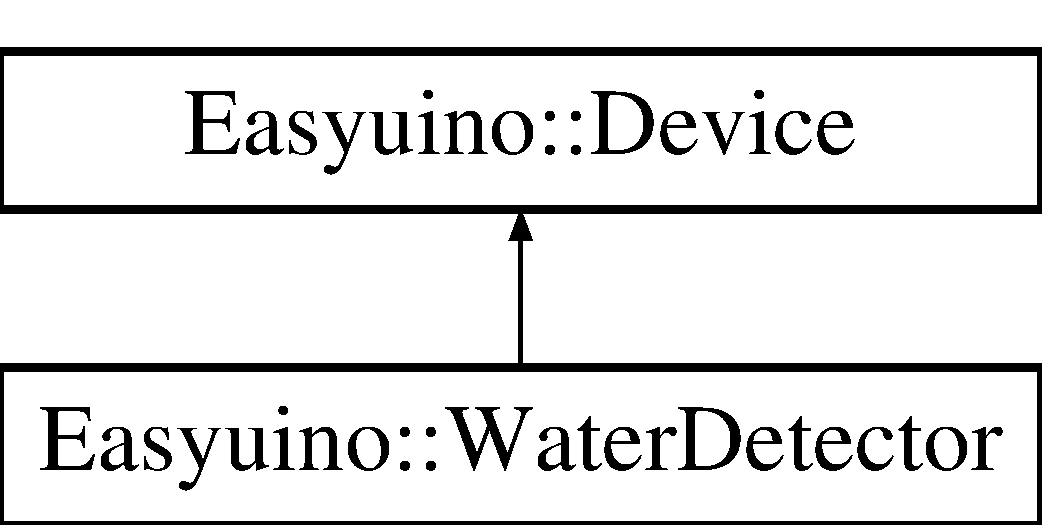
\includegraphics[height=2.000000cm]{class_easyuino_1_1_water_detector}
\end{center}
\end{figure}
\subsection*{Public Member Functions}
\begin{DoxyCompactItemize}
\item 
\hyperlink{class_easyuino_1_1_water_detector_a33690612b2b89efcfb97d4967b16c617}{Water\+Detector} (IN uint8\+\_\+t digital\+Pin, IN uint8\+\_\+t analog\+Pin)
\begin{DoxyCompactList}\small\item\em Constructor. \end{DoxyCompactList}\item 
\mbox{\Hypertarget{class_easyuino_1_1_water_detector_af63f706076f6941135412d57c1ddc5cf}\label{class_easyuino_1_1_water_detector_af63f706076f6941135412d57c1ddc5cf}} 
\hyperlink{class_easyuino_1_1_water_detector_af63f706076f6941135412d57c1ddc5cf}{$\sim$\+Water\+Detector} ()
\begin{DoxyCompactList}\small\item\em Destructor. \end{DoxyCompactList}\item 
bool \hyperlink{class_easyuino_1_1_water_detector_af7a0ec32d6abcb8c1060f493525d5228}{begin} ()
\begin{DoxyCompactList}\small\item\em Used to put the device ready to receive requests. \end{DoxyCompactList}\item 
bool \hyperlink{class_easyuino_1_1_water_detector_a06ac56298c56026691d7d6a9dbb63748}{begin} (IN uint8\+\_\+t digital\+Pin\+Trigger\+Level)
\begin{DoxyCompactList}\small\item\em Initialize the \hyperlink{class_easyuino_1_1_water_detector}{Water\+Detector} A\+PI putting it ready to receive requests. \end{DoxyCompactList}\item 
void \hyperlink{class_easyuino_1_1_water_detector_a9c1473536f47b2a7d8e1f8fb1bf5f3fd}{end} ()
\begin{DoxyCompactList}\small\item\em Used to stop the device A\+PI. \end{DoxyCompactList}\item 
Water\+Status \hyperlink{class_easyuino_1_1_water_detector_a0dfefd3b3aa2ed21f30ceb8041a8652a}{get\+Water\+Status} ()
\begin{DoxyCompactList}\small\item\em Returns an enumerate value depending on how wet is the sensor. \end{DoxyCompactList}\item 
unsigned int \hyperlink{class_easyuino_1_1_water_detector_a4a4c4a0ab6ae8a51535762f38b4f0d01}{get\+Water\+Status\+Range} ()
\begin{DoxyCompactList}\small\item\em Return a number in \mbox{[}0,1023\mbox{]} depending on dry is the sensor. \end{DoxyCompactList}\item 
bool \hyperlink{class_easyuino_1_1_water_detector_a9ea69c2eec25543fad47759379d62ce6}{is\+Water\+Detected} ()
\begin{DoxyCompactList}\small\item\em Used to get the value from the digital pin that is activated when a wet threshold is passed. \end{DoxyCompactList}\end{DoxyCompactItemize}
\subsection*{Additional Inherited Members}


\subsection{Detailed Description}
Rain\+Detector A\+PI is used to detect the amount of water that is touching the sensor. 



\subsection{Constructor \& Destructor Documentation}
\mbox{\Hypertarget{class_easyuino_1_1_water_detector_a33690612b2b89efcfb97d4967b16c617}\label{class_easyuino_1_1_water_detector_a33690612b2b89efcfb97d4967b16c617}} 
\index{Easyuino\+::\+Water\+Detector@{Easyuino\+::\+Water\+Detector}!Water\+Detector@{Water\+Detector}}
\index{Water\+Detector@{Water\+Detector}!Easyuino\+::\+Water\+Detector@{Easyuino\+::\+Water\+Detector}}
\subsubsection{\texorpdfstring{Water\+Detector()}{WaterDetector()}}
{\footnotesize\ttfamily Easyuino\+::\+Water\+Detector\+::\+Water\+Detector (\begin{DoxyParamCaption}\item[{IN uint8\+\_\+t}]{digital\+Pin,  }\item[{IN uint8\+\_\+t}]{analog\+Pin }\end{DoxyParamCaption})}



Constructor. 


\begin{DoxyParams}{Parameters}
{\em digital\+Pin} & Arduino pin connected to digital pin (Normally D0 in sensor board) \\
\hline
{\em analog\+Pin} & Arduino pin connected to analog pin (Normally A0 in sensor board) \\
\hline
\end{DoxyParams}


\subsection{Member Function Documentation}
\mbox{\Hypertarget{class_easyuino_1_1_water_detector_af7a0ec32d6abcb8c1060f493525d5228}\label{class_easyuino_1_1_water_detector_af7a0ec32d6abcb8c1060f493525d5228}} 
\index{Easyuino\+::\+Water\+Detector@{Easyuino\+::\+Water\+Detector}!begin@{begin}}
\index{begin@{begin}!Easyuino\+::\+Water\+Detector@{Easyuino\+::\+Water\+Detector}}
\subsubsection{\texorpdfstring{begin()}{begin()}\hspace{0.1cm}{\footnotesize\ttfamily [1/2]}}
{\footnotesize\ttfamily bool Easyuino\+::\+Water\+Detector\+::begin (\begin{DoxyParamCaption}{ }\end{DoxyParamCaption})\hspace{0.3cm}{\ttfamily [virtual]}}



Used to put the device ready to receive requests. 

Normally this have some default behaviour some devices have other overload method with same name that receives other arguments to device customization. \begin{DoxyReturn}{Returns}
True\+: If the device was initialized. False\+: Otherwise. 
\end{DoxyReturn}


Implements \hyperlink{class_easyuino_1_1_device_a2e7bb2fec849719a9d9432b57cdb72ba}{Easyuino\+::\+Device}.

\mbox{\Hypertarget{class_easyuino_1_1_water_detector_a06ac56298c56026691d7d6a9dbb63748}\label{class_easyuino_1_1_water_detector_a06ac56298c56026691d7d6a9dbb63748}} 
\index{Easyuino\+::\+Water\+Detector@{Easyuino\+::\+Water\+Detector}!begin@{begin}}
\index{begin@{begin}!Easyuino\+::\+Water\+Detector@{Easyuino\+::\+Water\+Detector}}
\subsubsection{\texorpdfstring{begin()}{begin()}\hspace{0.1cm}{\footnotesize\ttfamily [2/2]}}
{\footnotesize\ttfamily bool Easyuino\+::\+Water\+Detector\+::begin (\begin{DoxyParamCaption}\item[{IN uint8\+\_\+t}]{digital\+Pin\+Trigger\+Level }\end{DoxyParamCaption})}



Initialize the \hyperlink{class_easyuino_1_1_water_detector}{Water\+Detector} A\+PI putting it ready to receive requests. 


\begin{DoxyParams}{Parameters}
{\em digital\+Pin\+Trigger\+Level} & The digital level that is triggered in digital pin when water is sensed. \\
\hline
\end{DoxyParams}
\begin{DoxyReturn}{Returns}
True\+: If the device was initialized. False\+: Otherwise. 
\end{DoxyReturn}
\mbox{\Hypertarget{class_easyuino_1_1_water_detector_a9c1473536f47b2a7d8e1f8fb1bf5f3fd}\label{class_easyuino_1_1_water_detector_a9c1473536f47b2a7d8e1f8fb1bf5f3fd}} 
\index{Easyuino\+::\+Water\+Detector@{Easyuino\+::\+Water\+Detector}!end@{end}}
\index{end@{end}!Easyuino\+::\+Water\+Detector@{Easyuino\+::\+Water\+Detector}}
\subsubsection{\texorpdfstring{end()}{end()}}
{\footnotesize\ttfamily void Easyuino\+::\+Water\+Detector\+::end (\begin{DoxyParamCaption}{ }\end{DoxyParamCaption})\hspace{0.3cm}{\ttfamily [virtual]}}



Used to stop the device A\+PI. 

After this the the device will not process A\+PI requests. 

Implements \hyperlink{class_easyuino_1_1_device_ab31018ef64adc84aa2ea575b2297548f}{Easyuino\+::\+Device}.

\mbox{\Hypertarget{class_easyuino_1_1_water_detector_a0dfefd3b3aa2ed21f30ceb8041a8652a}\label{class_easyuino_1_1_water_detector_a0dfefd3b3aa2ed21f30ceb8041a8652a}} 
\index{Easyuino\+::\+Water\+Detector@{Easyuino\+::\+Water\+Detector}!get\+Water\+Status@{get\+Water\+Status}}
\index{get\+Water\+Status@{get\+Water\+Status}!Easyuino\+::\+Water\+Detector@{Easyuino\+::\+Water\+Detector}}
\subsubsection{\texorpdfstring{get\+Water\+Status()}{getWaterStatus()}}
{\footnotesize\ttfamily Water\+Status Easyuino\+::\+Water\+Detector\+::get\+Water\+Status (\begin{DoxyParamCaption}{ }\end{DoxyParamCaption})}



Returns an enumerate value depending on how wet is the sensor. 

\begin{DoxyReturn}{Returns}
water\+Status Available options in Water\+Status enumerate. 
\end{DoxyReturn}
\mbox{\Hypertarget{class_easyuino_1_1_water_detector_a4a4c4a0ab6ae8a51535762f38b4f0d01}\label{class_easyuino_1_1_water_detector_a4a4c4a0ab6ae8a51535762f38b4f0d01}} 
\index{Easyuino\+::\+Water\+Detector@{Easyuino\+::\+Water\+Detector}!get\+Water\+Status\+Range@{get\+Water\+Status\+Range}}
\index{get\+Water\+Status\+Range@{get\+Water\+Status\+Range}!Easyuino\+::\+Water\+Detector@{Easyuino\+::\+Water\+Detector}}
\subsubsection{\texorpdfstring{get\+Water\+Status\+Range()}{getWaterStatusRange()}}
{\footnotesize\ttfamily unsigned int Easyuino\+::\+Water\+Detector\+::get\+Water\+Status\+Range (\begin{DoxyParamCaption}{ }\end{DoxyParamCaption})}



Return a number in \mbox{[}0,1023\mbox{]} depending on dry is the sensor. 

Used in \hyperlink{class_easyuino_1_1_water_detector_a0dfefd3b3aa2ed21f30ceb8041a8652a}{get\+Water\+Status()} method. \begin{DoxyReturn}{Returns}
Number in range \mbox{[}0,1023\mbox{]}, 1023 = dry and 0 = flood or -\/1 if A\+PI is not initialized 
\end{DoxyReturn}
\mbox{\Hypertarget{class_easyuino_1_1_water_detector_a9ea69c2eec25543fad47759379d62ce6}\label{class_easyuino_1_1_water_detector_a9ea69c2eec25543fad47759379d62ce6}} 
\index{Easyuino\+::\+Water\+Detector@{Easyuino\+::\+Water\+Detector}!is\+Water\+Detected@{is\+Water\+Detected}}
\index{is\+Water\+Detected@{is\+Water\+Detected}!Easyuino\+::\+Water\+Detector@{Easyuino\+::\+Water\+Detector}}
\subsubsection{\texorpdfstring{is\+Water\+Detected()}{isWaterDetected()}}
{\footnotesize\ttfamily bool Easyuino\+::\+Water\+Detector\+::is\+Water\+Detected (\begin{DoxyParamCaption}{ }\end{DoxyParamCaption})}



Used to get the value from the digital pin that is activated when a wet threshold is passed. 

Normally the threshold is set using the potentiometer in the water detector board. \begin{DoxyReturn}{Returns}
True\+: If water threshold detection passed. False\+: Otherwise. 
\end{DoxyReturn}


The documentation for this class was generated from the following file\+:\begin{DoxyCompactItemize}
\item 
src/Water\+Detector.\+h\end{DoxyCompactItemize}

\hypertarget{class_water_detector_test}{}\section{Water\+Detector\+Test Class Reference}
\label{class_water_detector_test}\index{Water\+Detector\+Test@{Water\+Detector\+Test}}
Inheritance diagram for Water\+Detector\+Test\+:\begin{figure}[H]
\begin{center}
\leavevmode
\includegraphics[height=2.000000cm]{class_water_detector_test}
\end{center}
\end{figure}
\subsection*{Public Member Functions}
\begin{DoxyCompactItemize}
\item 
\mbox{\Hypertarget{class_water_detector_test_a22961d4d362a815532ba60c96d46ee4b}\label{class_water_detector_test_a22961d4d362a815532ba60c96d46ee4b}} 
{\bfseries Water\+Detector\+Test} (Stream \&debug\+Stream, uint8\+\_\+t digital\+Pin, uint8\+\_\+t analog\+Pin)
\end{DoxyCompactItemize}
\subsection*{Protected Member Functions}
\begin{DoxyCompactItemize}
\item 
\mbox{\Hypertarget{class_water_detector_test_ae7db8346c9f226ebb421e2b8e593cc7b}\label{class_water_detector_test_ae7db8346c9f226ebb421e2b8e593cc7b}} 
void {\bfseries tests\+Setup} ()
\item 
\mbox{\Hypertarget{class_water_detector_test_a85fcf9d1f00031b961bad2600ee54796}\label{class_water_detector_test_a85fcf9d1f00031b961bad2600ee54796}} 
void {\bfseries tests} ()
\item 
\mbox{\Hypertarget{class_water_detector_test_a18b0d5ee4b383e89a3e8a8ea2fd47e40}\label{class_water_detector_test_a18b0d5ee4b383e89a3e8a8ea2fd47e40}} 
void {\bfseries after\+Test\+Suite} ()
\end{DoxyCompactItemize}
\subsection*{Additional Inherited Members}


The documentation for this class was generated from the following file\+:\begin{DoxyCompactItemize}
\item 
src/tests/Water\+Detector\+Test.\+h\end{DoxyCompactItemize}

\hypertarget{class_easyuino_1_1_water_flow_meter}{}\section{Easyuino\+:\+:Water\+Flow\+Meter Class Reference}
\label{class_easyuino_1_1_water_flow_meter}\index{Easyuino\+::\+Water\+Flow\+Meter@{Easyuino\+::\+Water\+Flow\+Meter}}
Inheritance diagram for Easyuino\+:\+:Water\+Flow\+Meter\+:\begin{figure}[H]
\begin{center}
\leavevmode
\includegraphics[height=3.000000cm]{class_easyuino_1_1_water_flow_meter}
\end{center}
\end{figure}
\subsection*{Public Member Functions}
\begin{DoxyCompactItemize}
\item 
\mbox{\Hypertarget{class_easyuino_1_1_water_flow_meter_a253cbf06355c4e7dd79ef801d18c5119}\label{class_easyuino_1_1_water_flow_meter_a253cbf06355c4e7dd79ef801d18c5119}} 
{\bfseries Water\+Flow\+Meter} (IN uint8\+\_\+t sensor\+Pin)
\item 
bool \hyperlink{class_easyuino_1_1_water_flow_meter_a400c25b10a7cde45c623805546d071cd}{begin} ()
\begin{DoxyCompactList}\small\item\em Used to put the device ready to receive requests. \end{DoxyCompactList}\item 
void \hyperlink{class_easyuino_1_1_water_flow_meter_a47024d4da9568e42743a875c08c33121}{end} ()
\begin{DoxyCompactList}\small\item\em Used to stop the device A\+PI. \end{DoxyCompactList}\item 
\mbox{\Hypertarget{class_easyuino_1_1_water_flow_meter_a40e53d19dc4458bd149618053a52389f}\label{class_easyuino_1_1_water_flow_meter_a40e53d19dc4458bd149618053a52389f}} 
bool {\bfseries is\+Flowing} ()
\item 
\mbox{\Hypertarget{class_easyuino_1_1_water_flow_meter_a1798974218a55932876fafd749b98726}\label{class_easyuino_1_1_water_flow_meter_a1798974218a55932876fafd749b98726}} 
void {\bfseries update\+Flow\+Rate} ()
\item 
\mbox{\Hypertarget{class_easyuino_1_1_water_flow_meter_a3f531a6a6f8bf9a27d43915004889085}\label{class_easyuino_1_1_water_flow_meter_a3f531a6a6f8bf9a27d43915004889085}} 
float {\bfseries get\+Flow\+Rate} ()
\end{DoxyCompactItemize}
\subsection*{Additional Inherited Members}


\subsection{Member Function Documentation}
\mbox{\Hypertarget{class_easyuino_1_1_water_flow_meter_a400c25b10a7cde45c623805546d071cd}\label{class_easyuino_1_1_water_flow_meter_a400c25b10a7cde45c623805546d071cd}} 
\index{Easyuino\+::\+Water\+Flow\+Meter@{Easyuino\+::\+Water\+Flow\+Meter}!begin@{begin}}
\index{begin@{begin}!Easyuino\+::\+Water\+Flow\+Meter@{Easyuino\+::\+Water\+Flow\+Meter}}
\subsubsection{\texorpdfstring{begin()}{begin()}}
{\footnotesize\ttfamily bool Easyuino\+::\+Water\+Flow\+Meter\+::begin (\begin{DoxyParamCaption}{ }\end{DoxyParamCaption})\hspace{0.3cm}{\ttfamily [virtual]}}



Used to put the device ready to receive requests. 

Normally this have some default behaviour some devices have other overload method with same name that receives other arguments to device customization. \begin{DoxyReturn}{Returns}
True\+: If the device was initialized. False\+: Otherwise. 
\end{DoxyReturn}


Implements \hyperlink{class_easyuino_1_1_device_a2e7bb2fec849719a9d9432b57cdb72ba}{Easyuino\+::\+Device}.

\mbox{\Hypertarget{class_easyuino_1_1_water_flow_meter_a47024d4da9568e42743a875c08c33121}\label{class_easyuino_1_1_water_flow_meter_a47024d4da9568e42743a875c08c33121}} 
\index{Easyuino\+::\+Water\+Flow\+Meter@{Easyuino\+::\+Water\+Flow\+Meter}!end@{end}}
\index{end@{end}!Easyuino\+::\+Water\+Flow\+Meter@{Easyuino\+::\+Water\+Flow\+Meter}}
\subsubsection{\texorpdfstring{end()}{end()}}
{\footnotesize\ttfamily void Easyuino\+::\+Water\+Flow\+Meter\+::end (\begin{DoxyParamCaption}{ }\end{DoxyParamCaption})\hspace{0.3cm}{\ttfamily [virtual]}}



Used to stop the device A\+PI. 

After this the the device will not process A\+PI requests. 

Implements \hyperlink{class_easyuino_1_1_device_ab31018ef64adc84aa2ea575b2297548f}{Easyuino\+::\+Device}.



The documentation for this class was generated from the following file\+:\begin{DoxyCompactItemize}
\item 
src/Water\+Flow\+Meter.\+h\end{DoxyCompactItemize}

\hypertarget{class_easyuino_1_1_water_flow_sensor}{}\section{Easyuino\+:\+:Water\+Flow\+Sensor Class Reference}
\label{class_easyuino_1_1_water_flow_sensor}\index{Easyuino\+::\+Water\+Flow\+Sensor@{Easyuino\+::\+Water\+Flow\+Sensor}}
Inheritance diagram for Easyuino\+:\+:Water\+Flow\+Sensor\+:\begin{figure}[H]
\begin{center}
\leavevmode
\includegraphics[height=3.000000cm]{class_easyuino_1_1_water_flow_sensor}
\end{center}
\end{figure}
\subsection*{Public Member Functions}
\begin{DoxyCompactItemize}
\item 
\mbox{\Hypertarget{class_easyuino_1_1_water_flow_sensor_acee82d1863cb2311e58210906d9fbfaa}\label{class_easyuino_1_1_water_flow_sensor_acee82d1863cb2311e58210906d9fbfaa}} 
{\bfseries Water\+Flow\+Sensor} (IN uint8\+\_\+t sensor\+Pin)
\item 
bool \hyperlink{class_easyuino_1_1_water_flow_sensor_a55dcab6c527b1e1951a1fff69efdb763}{begin} ()
\begin{DoxyCompactList}\small\item\em Used to put the device ready to receive requests. \end{DoxyCompactList}\item 
void \hyperlink{class_easyuino_1_1_water_flow_sensor_a7f31ac7735b049394d34cfbc37f17359}{end} ()
\begin{DoxyCompactList}\small\item\em Used to stop the device A\+PI. \end{DoxyCompactList}\item 
\mbox{\Hypertarget{class_easyuino_1_1_water_flow_sensor_a677d164cb17c56407c8102662b0c3cd4}\label{class_easyuino_1_1_water_flow_sensor_a677d164cb17c56407c8102662b0c3cd4}} 
virtual bool {\bfseries is\+Flowing} ()
\end{DoxyCompactItemize}
\subsection*{Protected Member Functions}
\begin{DoxyCompactItemize}
\item 
\mbox{\Hypertarget{class_easyuino_1_1_water_flow_sensor_adc2ba2c1888114b01719cfd6a659d59b}\label{class_easyuino_1_1_water_flow_sensor_adc2ba2c1888114b01719cfd6a659d59b}} 
void {\bfseries enable\+Pulse\+Counting} ()
\item 
\mbox{\Hypertarget{class_easyuino_1_1_water_flow_sensor_a66d275227c18329b38f33834b4682ff3}\label{class_easyuino_1_1_water_flow_sensor_a66d275227c18329b38f33834b4682ff3}} 
void {\bfseries disable\+Pulse\+Couning} ()
\end{DoxyCompactItemize}
\subsection*{Protected Attributes}
\begin{DoxyCompactItemize}
\item 
\mbox{\Hypertarget{class_easyuino_1_1_water_flow_sensor_a7efef15ef9da3a66bd40183c4ea908ff}\label{class_easyuino_1_1_water_flow_sensor_a7efef15ef9da3a66bd40183c4ea908ff}} 
uint8\+\_\+t {\bfseries \+\_\+sensor\+Pin}
\item 
\mbox{\Hypertarget{class_easyuino_1_1_water_flow_sensor_a8877c5e4a3ed8012341d416ce05fa93e}\label{class_easyuino_1_1_water_flow_sensor_a8877c5e4a3ed8012341d416ce05fa93e}} 
volatile uint32\+\_\+t {\bfseries \+\_\+pulse\+Counter}
\end{DoxyCompactItemize}


\subsection{Member Function Documentation}
\mbox{\Hypertarget{class_easyuino_1_1_water_flow_sensor_a55dcab6c527b1e1951a1fff69efdb763}\label{class_easyuino_1_1_water_flow_sensor_a55dcab6c527b1e1951a1fff69efdb763}} 
\index{Easyuino\+::\+Water\+Flow\+Sensor@{Easyuino\+::\+Water\+Flow\+Sensor}!begin@{begin}}
\index{begin@{begin}!Easyuino\+::\+Water\+Flow\+Sensor@{Easyuino\+::\+Water\+Flow\+Sensor}}
\subsubsection{\texorpdfstring{begin()}{begin()}}
{\footnotesize\ttfamily bool Easyuino\+::\+Water\+Flow\+Sensor\+::begin (\begin{DoxyParamCaption}{ }\end{DoxyParamCaption})\hspace{0.3cm}{\ttfamily [virtual]}}



Used to put the device ready to receive requests. 

Normally this have some default behaviour some devices have other overload method with same name that receives other arguments to device customization. \begin{DoxyReturn}{Returns}
True\+: If the device was initialized. False\+: Otherwise. 
\end{DoxyReturn}


Implements \hyperlink{class_easyuino_1_1_device_a2e7bb2fec849719a9d9432b57cdb72ba}{Easyuino\+::\+Device}.

\mbox{\Hypertarget{class_easyuino_1_1_water_flow_sensor_a7f31ac7735b049394d34cfbc37f17359}\label{class_easyuino_1_1_water_flow_sensor_a7f31ac7735b049394d34cfbc37f17359}} 
\index{Easyuino\+::\+Water\+Flow\+Sensor@{Easyuino\+::\+Water\+Flow\+Sensor}!end@{end}}
\index{end@{end}!Easyuino\+::\+Water\+Flow\+Sensor@{Easyuino\+::\+Water\+Flow\+Sensor}}
\subsubsection{\texorpdfstring{end()}{end()}}
{\footnotesize\ttfamily void Easyuino\+::\+Water\+Flow\+Sensor\+::end (\begin{DoxyParamCaption}{ }\end{DoxyParamCaption})\hspace{0.3cm}{\ttfamily [virtual]}}



Used to stop the device A\+PI. 

After this the the device will not process A\+PI requests. 

Implements \hyperlink{class_easyuino_1_1_device_ab31018ef64adc84aa2ea575b2297548f}{Easyuino\+::\+Device}.



The documentation for this class was generated from the following file\+:\begin{DoxyCompactItemize}
\item 
src/Water\+Flow\+Sensor.\+h\end{DoxyCompactItemize}

%--- End generated contents ---

% Index
\backmatter
\newpage
\phantomsection
\clearemptydoublepage
\addcontentsline{toc}{chapter}{Index}
\printindex

\end{document}
